% Options for packages loaded elsewhere
\PassOptionsToPackage{unicode}{hyperref}
\PassOptionsToPackage{hyphens}{url}
%
\documentclass[
  12pt,
]{book}
\usepackage{amsmath,amssymb}
\usepackage{lmodern}
\usepackage{iftex}
\ifPDFTeX
  \usepackage[T1]{fontenc}
  \usepackage[utf8]{inputenc}
  \usepackage{textcomp} % provide euro and other symbols
\else % if luatex or xetex
  \usepackage{unicode-math}
  \defaultfontfeatures{Scale=MatchLowercase}
  \defaultfontfeatures[\rmfamily]{Ligatures=TeX,Scale=1}
  \setmainfont[]{Times New Roman}
\fi
% Use upquote if available, for straight quotes in verbatim environments
\IfFileExists{upquote.sty}{\usepackage{upquote}}{}
\IfFileExists{microtype.sty}{% use microtype if available
  \usepackage[]{microtype}
  \UseMicrotypeSet[protrusion]{basicmath} % disable protrusion for tt fonts
}{}
\makeatletter
\@ifundefined{KOMAClassName}{% if non-KOMA class
  \IfFileExists{parskip.sty}{%
    \usepackage{parskip}
  }{% else
    \setlength{\parindent}{0pt}
    \setlength{\parskip}{6pt plus 2pt minus 1pt}}
}{% if KOMA class
  \KOMAoptions{parskip=half}}
\makeatother
\usepackage{xcolor}
\IfFileExists{xurl.sty}{\usepackage{xurl}}{} % add URL line breaks if available
\IfFileExists{bookmark.sty}{\usepackage{bookmark}}{\usepackage{hyperref}}
\hypersetup{
  pdftitle={History of the Piedmont Neighborhood until 1920},
  pdfauthor={Jan de Leeuw},
  hidelinks,
  pdfcreator={LaTeX via pandoc}}
\urlstyle{same} % disable monospaced font for URLs
\usepackage{longtable,booktabs,array}
\usepackage{calc} % for calculating minipage widths
% Correct order of tables after \paragraph or \subparagraph
\usepackage{etoolbox}
\makeatletter
\patchcmd\longtable{\par}{\if@noskipsec\mbox{}\fi\par}{}{}
\makeatother
% Allow footnotes in longtable head/foot
\IfFileExists{footnotehyper.sty}{\usepackage{footnotehyper}}{\usepackage{footnote}}
\makesavenoteenv{longtable}
\usepackage{graphicx}
\makeatletter
\def\maxwidth{\ifdim\Gin@nat@width>\linewidth\linewidth\else\Gin@nat@width\fi}
\def\maxheight{\ifdim\Gin@nat@height>\textheight\textheight\else\Gin@nat@height\fi}
\makeatother
% Scale images if necessary, so that they will not overflow the page
% margins by default, and it is still possible to overwrite the defaults
% using explicit options in \includegraphics[width, height, ...]{}
\setkeys{Gin}{width=\maxwidth,height=\maxheight,keepaspectratio}
% Set default figure placement to htbp
\makeatletter
\def\fps@figure{htbp}
\makeatother
\setlength{\emergencystretch}{3em} % prevent overfull lines
\providecommand{\tightlist}{%
  \setlength{\itemsep}{0pt}\setlength{\parskip}{0pt}}
\setcounter{secnumdepth}{5}
\ifLuaTeX
  \usepackage{selnolig}  % disable illegal ligatures
\fi

\title{History of the Piedmont Neighborhood until 1920}
\author{Jan de Leeuw}
\date{Started in 2016. Last update August 30, 2021}

\begin{document}
\maketitle

{
\setcounter{tocdepth}{4}
\tableofcontents
}
\begin{figure}
\centering
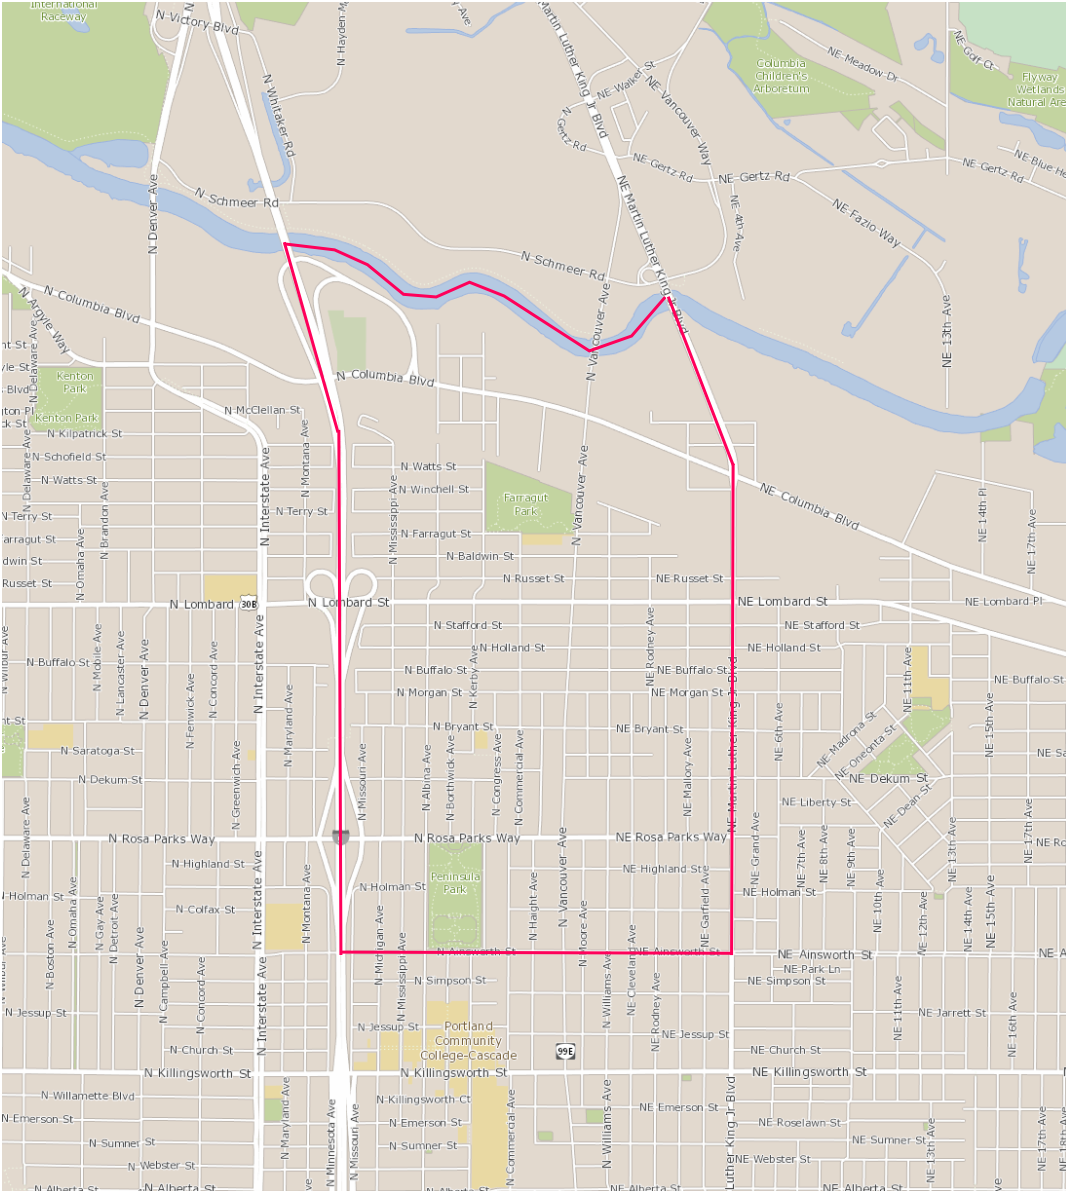
\includegraphics{index/images/image1.png}
\caption{alt\_text}
\end{figure}

\begin{enumerate}
\def\labelenumi{\arabic{enumi}.}
\setcounter{enumi}{-1}
\item
  Introduction \href{https://drive.google.com/open?id=1QzHMQrMUnutETlBx5yGboK6RO50koiM_}{{[}PDF{]}}
\item
  They Were Here First -- And They Are Still Here \href{https://drive.google.com/open?id=1kWwwu8cXTcRqNVLZfDET9bZqTH_VN13UUYbacRjDL9M}{{[}PDF{]}}
\item
  Homesteaders and Homesteads

\begin{verbatim}
   2.00 Introduction [[PDF]](https://drive.google.com/open?id=1WROfaTYwgUjKMKHpcGhDY0z83CBWSP6N)
\end{verbatim}
\end{enumerate}

2.01 Evander Howe \href{https://drive.google.com/open?id=1YAycX-_hJXmEAvgMUgpsdMuTcHbiE48o}{{[}PDF{]}}

2.02 George and Elizabeth Smith \href{https://drive.google.com/open?id=1AAWNbZ1PpfN6j8m0dtyi9sBDhvlUTULD}{{[}PDF{]}}

2.03 Lewis and Nancy Love \href{https://drive.google.com/open?id=1Jv2GCT7bdq1UjKnJm2y1qHjyfE3epBMg}{{[}PDF{]}}

2.04 David and Martha Ulery \href{https://drive.google.com/open?id=1T59_j3N5wUB8kfVnfxyKY33XiNLHroEn}{{[}PDF{]}}

2.05 John Fenstermacher \href{https://drive.google.com/open?id=10M9wj9ehPJ7G1Ga6Z3WUreQJwETT1NW3}{{[}PDF{]}}

\begin{enumerate}
\def\labelenumi{\arabic{enumi}.}
\setcounter{enumi}{2}
\tightlist
\item
  Subdivisions
\end{enumerate}

3.00 Introduction

3.01 Beverly

3.02 Cumberland

3.03 Devine's Addition

3.04 Fairport

3.05 Gainsborough \href{https://drive.google.com/open?id=1-yUUA6gAcEnZ6JcIE4JlhUdyhjZH-XkU}{{[}PDF{]}}

3.06 Gem Addition to Albina

3.07 Gerard Addition

3.08 Green C Love Addition

3.09 Kirkmar \href{https://drive.google.com/open?id=1K0Vy_pLA6v6lHOG20JHfW3pFNbB_y_As}{{[}PDF{]}}

3.10 Lahoma

3.11 Lochinvar \href{https://drive.google.com/open?id=1WYFm9L-zLTn4d3Z-P0jHR7H764vB_IzJ}{{[}PDF{]}}

3.12 Longview

3.13 Loveleigh \href{https://drive.google.com/open?id=124KTO88KNKYI06S_Kg7mD37j-HojvKZM}{{[}PDF{]}}

3.14 Lovewood \href{https://drive.google.com/open?id=1MFAF_zvS91iEljKEif22ZFuFzNk1NBpg}{{[}PDF{]}}

3.15 Love's Addition

3.16 New Albina

3.17 Newmarket Row

3.18 Nocera

3.19 Pacific Place

3.20 Parkway

3.21 Piedmont \href{https://l.facebook.com/l.php?u=https\%3A\%2F\%2Fdrive.google.com\%2Fopen\%3Fid\%3D1-9EhdqV51Y03rqUdg9TRgpD-xLiKQvQi\&h=AT3nGsWmXhbQfW9A2d5Qky-O-fy3KsvekepBBd3uEGmoKh0FijpfGT5DpcKsh9-Zt3b2c2v5TnvZ4ddoydn__lb0fA8blySjjnTpQJMzTyYehW2h8JKgDHUh6LYYn_FT-2k1soRzIMc_VGwykcrQHuQRtj1lPaUXkcXBm2k-O_BKdi2HIy7qkHaOH5QPDc3bSqJrKkswdXNRDIUDjrPKAVujS-IMBTKFVtWCKVJEpSgFFfAKkLTlAE5VbJtspKZm0xzSrmJQlieHyWLnEaTGcXlaNmw_BdWhE118AcHAfb1ZybOS0suTqJibOPbAhIOZILkK2Q5GJD38IKvigNVa-f2CDPw724oLFtG4Rkig7ErCQRaAdVf0vdZy2aNrTm2zg8JlxyrXLuMusgNtmo3HhQ}{{[}PDF{]}}

3.22 Piedmont Park

3.23 Rose Addition

3.24 Saratoga \href{https://drive.google.com/open?id=1OHx5hx1NCU-MoAAo68ppMKhZgD1GoYKn}{{[}PDF{]}}

3.25 Swinton

\begin{enumerate}
\def\labelenumi{\arabic{enumi}.}
\setcounter{enumi}{3}
\tightlist
\item
  Structures
\end{enumerate}

4.01 Peninsula Park\href{https://drive.google.com/open?id=1fdXTV5QR_LCgfULxlq1tuFWetOSDZWXF}{{[}PDF{]}}

\begin{verbatim}
        4.02 Farragut Park [[PDF]](https://drive.google.com/open?id=10p9zhBn2-Tl7tPaFFjruxsn0u4Hq34Bh)
\end{verbatim}

4.03 Rankin Airport \href{https://drive.google.com/open?id=18IhFuHFxIyZp1qiESwfkOsqlK6fmfQnH}{{[}PDF{]}}

4.04 Municipal Car Park \href{https://drive.google.com/open?id=0B94Urj3OjM7BeTBxSGwwVW5kZ0E}{{[}PDF{]}}

\begin{verbatim}
        4.06 Lombard Theater [[PDF]](https://drive.google.com/open?id=1AGa31DL-i8ILhVhVp_4H24ZlfFAjCZ1b)
\end{verbatim}

4.05 Ockley Green School \href{https://drive.google.com/open?id=17Du1TnGsbrWakfCaSi3X1GP-bNSK16Xi}{{[}PDF{]}}

4.06 Vanport

4.07 Portland International Raceway

4.08 Portland Meadows

4.09 Columbia Cemetery

4.10 Minnesota Freeway

4.11 Peninsula Park Commons

4.12 Rosemont Commons

4.13 Holy Redeemer

4.14 The Swift Plant

\begin{enumerate}
\def\labelenumi{\arabic{enumi}.}
\setcounter{enumi}{4}
\item
  Homes

\begin{verbatim}
     5.01 Introduction [[PDF]](https://drive.google.com/open?id=1258hXyiSmeJexTZ5kETJbT3AuhvQoC0B)
\end{verbatim}

  5.02 8 North Stafford Street \href{https://drive.google.com/open?id=1njP7hB8vLeHYKtBuj5woXO30exj63RsC}{{[}PDF{]}}

\begin{verbatim}
     5.03 107 Northeast Bryant Street [[PDF]](https://drive.google.com/open?id=1V0GEeHTIvC4QfW-6gj3qiGiERnXb97i2)
\end{verbatim}
\item
  Streets
\end{enumerate}

6.01 The Road to Vancouver \href{https://drive.google.com/open?id=1cRbmNIRf3RuNY-YTFR6RlJn9syr2wQ7I}{{[}PDF{]}}

\begin{verbatim}
        6.02 The Peninsula Boulevard System [[PDF]](https://drive.google.com/open?id=1uzND2wmMkJsib1O4zYNCOBy2y0zTM3n6)
\end{verbatim}

6.03 Portland Boulevard/Rosa Parks Way \href{https://drive.google.com/open?id=1C1D7t9tRfvBke_81-sVMeE-cfmPuh3gG}{{[}PDF{]}}

6.04 Union Avenue/Martin Luther King Jr Boulevard \href{https://drive.google.com/open?id=14O557QNs9NU-0t7JLnDv3JiS37QhmOze}{{[}PDF{]}}

6.05 Williams Avenue

6.06 Ainsworth Street

6.07 Lombard Street

6.08 Columbia Boulevard

6.09 Bryant Street

6.10 Albina Avenue

\begin{enumerate}
\def\labelenumi{\arabic{enumi}.}
\setcounter{enumi}{6}
\item
  Streetcars and Railroads

\begin{verbatim}
     7.01 Introduction [[PDF]](https://drive.google.com/open?id=1ZW5GjsUc4VbwUHtGqBzJumZhYINavC2E)

     7.02 Vancouver

     7.03 St. Johns

     7.04 Williams
\end{verbatim}
\end{enumerate}

7.05 Mississippi

\begin{verbatim}
        7.06 Railways
\end{verbatim}

7.07 The Piedmont Car Barns

\begin{enumerate}
\def\labelenumi{\arabic{enumi}.}
\setcounter{enumi}{7}
\tightlist
\item
  Miscellaneous Persons
\end{enumerate}

8.01 Liverpool Liz, the Senate Saloon, and Evergreen Park \href{https://drive.google.com/open?id=1XRryQ5xFXDOjHw9p7dL2TDQ8LO6sDVY7}{{[}PDF{]}}

8.02 William Kanan Smith \href{https://drive.google.com/open?id=11IYZqK6zaRPzNa72t1B9tkQfkhWjxb5Q}{{[}PDF{]}}

8.03 Edward Quackenbush

\begin{verbatim}
        8.04 John Hotts

        8.05 John and Elizabeth Rankin
\end{verbatim}

8.06 Francis I. McKenna

8.07 H. C. Wortman

8.08 The Martin Family \href{https://drive.google.com/open?id=1mADoFI29ftPLipamI5EpRdigcEXK-rRr}{{[}PDF{]}}

8.09 The Love Family \href{https://drive.google.com/file/d/12YJDhcY3dOTeGUjoitX8C6pLar2bG9-C}{{[}PDF{]}}

8.10 Sylvester Farrell \href{https://drive.google.com/open?id=1O9K2LZWhjggLN-gjY8EIPYTNptBFcFWn}{{[}PDF{]}}

8.11 Elias Brong \href{https://drive.google.com/open?id=1KCOXqU17d8_UfDC7sHdCaGlExHLG8tVt}{{[}PDF{]}}

8.12 The Marshall Family

8.13 The McMillen Family

8.14 Gustave and Amelia Keller

\hypertarget{introduction-version-10022020}{%
\chapter{Introduction (Version 10/02/2020)}\label{introduction-version-10022020}}

\hypertarget{piedmont}{%
\section{Piedmont}\label{piedmont}}

Piedmont is one of the 95 neighborhoods in the neighborhood system of Portland, Oregon, and one of the eleven neighborhoods in the North Portland district coalition.

\begin{quote}
\emph{Portland's nationally recognized neighborhood system is made up of 95 recognized,
independent neighborhood associations and seven neighborhood district coalition offices
that represent the entire city of Portland.
\url{https://www.portlandoregon.gov/oni/28989}}
\end{quote}

The Piedmont neighborhood gets its name from the Piedmont subdivision, platted in 1889 by Edward Quackenbush and the Investment Company. And the Piedmont subdivision gets its name from the region in northwest Italy, known for its gentle slopes and hillsides. I am pretty sure the name Piedmont was chosen for its commercial appeal, and not for the physical resemblance with the eponymous region in Italy, which actually looks quite different.

Although:\url{https://en.wikipedia.org/wiki/Piedmont_(United_States)}

The Piedmont subdivision is only a small part of the Piedmont neighborhood, in fact less than ten percent of its area. And, conversely, only half of the Piedmont subdivision is in the Piedmont neighborhood, the rest is in Humboldt and King.

\hypertarget{land}{%
\section{Land}\label{land}}

Throughout this book, I concentrate on land and land ownership. It is essential, therefore, to remember that Oregon, Portland, and Piedmont were started by settler colonialism. This meant the United States occupied lands used for centuries by indigenous peoples, and declared it to be public lands of the United States. War, terror, vigilantes, disease, broken treaties, racism, religion, and unjust laws made sure the unceded lands stayed in the hands of the occupying forces. The small percentage of indigenous people that survived the onslaught were driven onto ever shrinking reservations. In the middle of the nineteenth century, when settlers started to arrive and Portland became a fast growing city, there were very few Native Americans left in the area.

In that nineteenth century the United States adopted laws which encouraged settlement by giving large sections of public lands away (usually tracts of 160 acres), and making other sections available for very little money (usually for \$ 1.25 per acre). The land that currently makes up Piedmont was donated in this way to just four people. Evander Howe, George Smith, Lewis Love, and David Ulery were all farmers on the Vancouver Road, near the Columbia Slough. They could effectively use the Donation Land Claim Act and the Military Bounty Law, because they were the first settlers to arrive, and actually for quite some time the only settlers to arrive.

In the next stage the city grew because the settlers, or ``pioneers'', sold their land to developers, who platted subdivisions. Piedmont over the years became differentiated from about four homesteads to about 30 subdivisions of varying sizes. From 1850 on fortunes were made by subdividing, exchanging, transfering, inheriting, buying, and selling pieces of land. In the third stage of development each of the subdivisions, sometimes also called additions, were partitioned into a varying number of city blocks, usually 200 by 200 feet, and the blocks were partitioned in lots, usually eight lots of 100 by 50 feet. These individual lots were then sold to people to build their houses, or packaged into multiple lots for speculation. Piedmont consists of thousands of such lots.

In the book I will discuss the original homesteads and the subsequent subdivisions. As a consequence of this emphasis on land, the book concentrates on the time between 1850 and 1930. After 1930 development is mostly down to the level of individual lots, and since there are about 5000 of these, I cannot discuss them one by one. It is interesting, of course, to find out who built an individual house, and who the subsequent owners were. But the sheer number of them makes it impossible to write about each and every one.

\hypertarget{bias}{%
\section{Bias}\label{bias}}

As you will probably figure out quickly, I like maps. I also like facts, more than I like opinions. I like words, more than I like photographs. Thus this book is not of the coffee table type, with many photos and only a few words.

I also do not like the view that historical developments are driven by a small number of important individuals, always men of course, and that we want to know as much as possible about these men, possibly because we want to become just like them. History is driven by social and economic forces and movements in which specific individuals are of limited and largely anecdotal significance. I like to report about structures and systems more than I like to report about people. Also, I hope that what I do report about the men and women that were important in Piedmont's early history makes it clear that you do not necessarily want to become just like them.

There are two other important types of Portland history books I do not want to emulate. Some of them are excellent, but they are not what I am interested in. There are those books that concentrate on vice, corruption, crime, shanghaiing, and prostitution. They are mostly about the northwest of Portland, between 1870 and 1910. And then there are those books that tell the story of city government and the business community, again mostly although not entirely about the part of Portland west of the river. As far as I am concerned, these two types of books talk about two sides of the same coin, a bunch of people quibbling on how to divide the loot. Of course that describes a huge part of history in general, and in this book the loot is basically two square miles of land, sections 10 and 15 in township one north, range one east of the Willamette Meridian.

\hypertarget{technical}{%
\section{Technical}\label{technical}}

This book is, and always will be, free and in the public domain. Anyone can copy, print, distribute or otherwise use the material in this book for any purpose whatsoever, and, if they so choose, without attribution.

All references are collected in the back of each chapter or section. I have tried to make everything reproducible, in the sense that every statement of fact that I make can be traced back to its sources. I have also tried to emphasize primary (i.e.~contemporaneous) sources, even if they were only newspaper articles. Secondary sources are only used, reluctantly, if primary sources are not available. I have also tried to refrain, as much as is humanly possible, from stating opinions about events, or making inferences about motives.

This book is a living document, which means that any part of it can change at any moment. Thus all sections have a date attached to their title, indicating when they were last changed. I keep discovering new facts and adding new materials. In the table of contents each section is linked to a separate pdf, which is synchronized with the sections in the Google docs version of the book.

This book is also, among other things, a repository. There are copies of, or links to, the original maps, deeds, photos, and newspaper articles that the narrative is based on. If you see a link below a figure or a map, then following that link will usually get you to a bigger and better version of the map you can either download to your computer or view in your browser. Generally you get the best resolution by downloading the file and opening it in the appropriate application.

\hypertarget{references}{%
\chapter{References}\label{references}}

The City of Portland, Oregon. \emph{Neighborhood Program.}

\url{https://www.portlandoregon.gov/oni/28989}

Alta Mitchoff: \emph{History of the Kenton Neighborhood}

Kenton Neighborhood Association, 1997

Anjala Ehelebe:\_ Portland's Woodlawn Neighborhood\_

Arcadia Publishing, 2008

Roy E. Roos: \emph{The History and Development of Portland's Irvington Neighborhood}

Self published, 1997

Roy E. Roos: \emph{The History of Albina. Including Eliot, Boise, King, Humboldt, and Piedmont Neighborhoods.}

Self published, 2008

Homes: 8 North Stafford Street and Environs

Jan de Leeuw

Version 02-09-2020

\begin{figure}
\centering
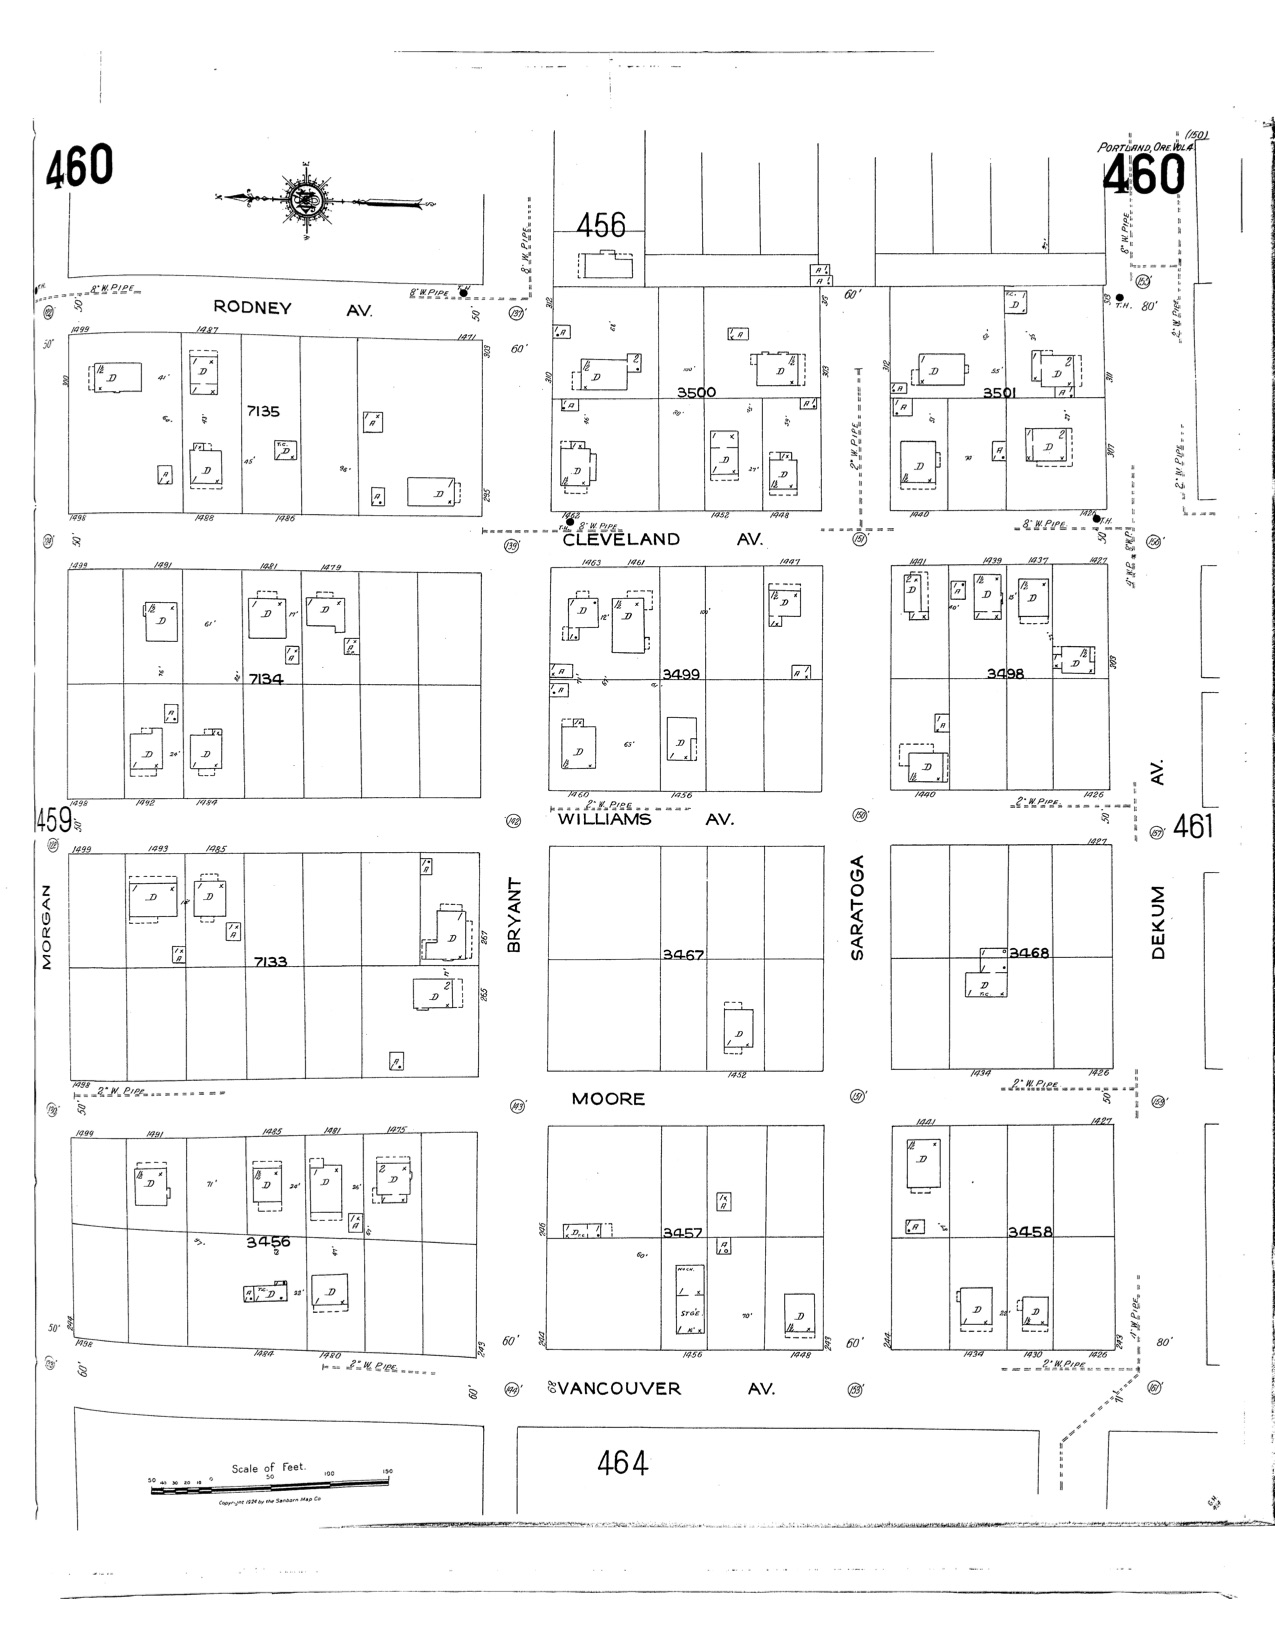
\includegraphics{images/image1.jpg}
\caption{alt\_text}
\end{figure}

Table of Contents

{[}TOC{]}

Introduction

This chapter will be about the house that we (Nicole and Jan) bought in 2014, when we moved to Portland from California. It may not be particularly interesting to others, but please indulge me. Here is the location of our house on Portland Maps. It is on the southwest corner of the intersection of Stafford Street and Williams Avenue, with address 8 North Stafford Street.

Williams Avenue is the dividing line between North and Northeast Portland, which explains the low street number. Also note that the house on the other side of Williams has a Williams Avenue address. More about that later.

{\textgreater\textgreater\textgreater\textgreater\textgreater{} gd2md-html alert: inline image link here (to images/image2.png). Store image on your image server and adjust path/filename/extension if necessary. }(Back to top)(Next alert){\textgreater\textgreater\textgreater\textgreater\textgreater{} }

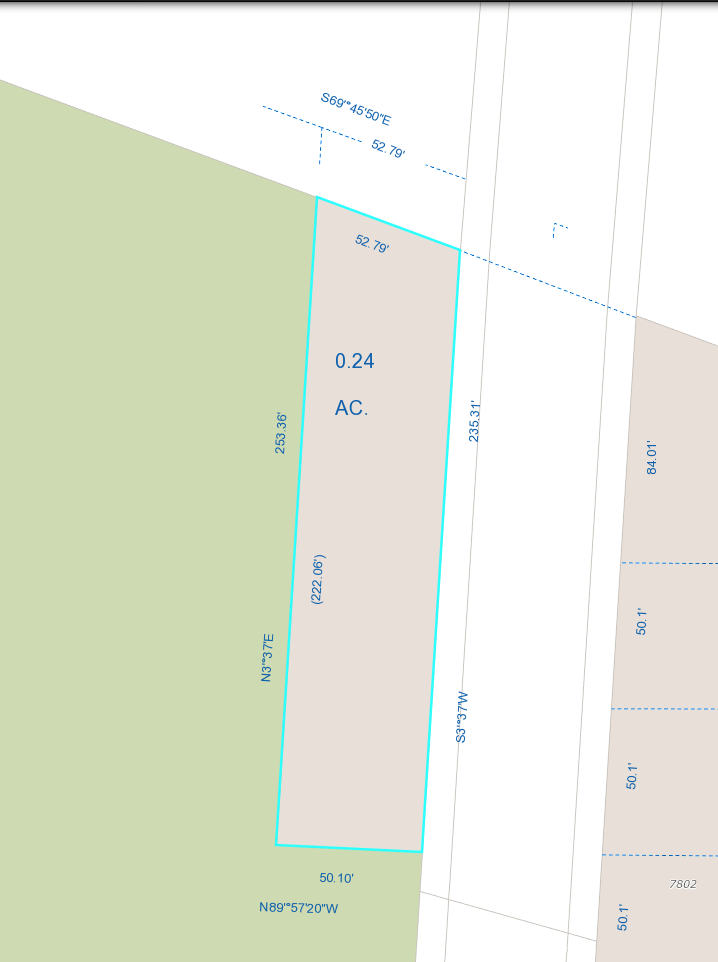
\includegraphics{images/image2.png}

Land

When Captain Lewis Love died in 1903 his 750 acres in the (what is now) Piedmont and Woodlawn neighborhoods were partitioned into six vertical strips, one for each of his six children (or their heirs, in case they were deceased). One of these strips was between Vancouver Avenue and Rodney Avenue, from Bryant Street in the south to the Columbia Slough in the north, totalling about 150 acres. It included the eastern half of Vancouver Avenue, which was just a right of way, not a city street, at the time. It went to the heirs of the oldest son, William Love, who had died in 1879. William Love had five children, so each of them inherited a 1/30 part of the Love estate.

One of the provisions in the will was that the heirs could not take possession of the land until January 1, 1907. This was too long a wait for some of the more impatient younger Loves, and one of William's sons sold his 1/30 part of the estate in 1904 to D.J. Buckley for \$ 10,000. On March 10, 1908 the remaining heirs, and Buckley, sold the lower half of the strip, the 50.49 acres between the Oregon Railway and Navigation Company's right of way and Bryant Street, to Elias Brong for \$ 63,075. The 101 acres of the same strip north of the railway were sold a year later by the same parties to the Columbia Trust Company.

Plat

On March 27,1908 the Brong-Steele Company recorded the plat for Loveleigh, which was 50.49 acres with Vancouver Avenue and 48.68 acres without Vancouver Avenue. The map shows the 20 city blocks that were laid out, with a total of 320 lots. Our house is on lot 12 in block 6.

{\textgreater\textgreater\textgreater\textgreater\textgreater{} gd2md-html alert: inline image link here (to images/image3.png). Store image on your image server and adjust path/filename/extension if necessary. }(Back to top)(Next alert){\textgreater\textgreater\textgreater\textgreater\textgreater{} }

\begin{figure}
\centering
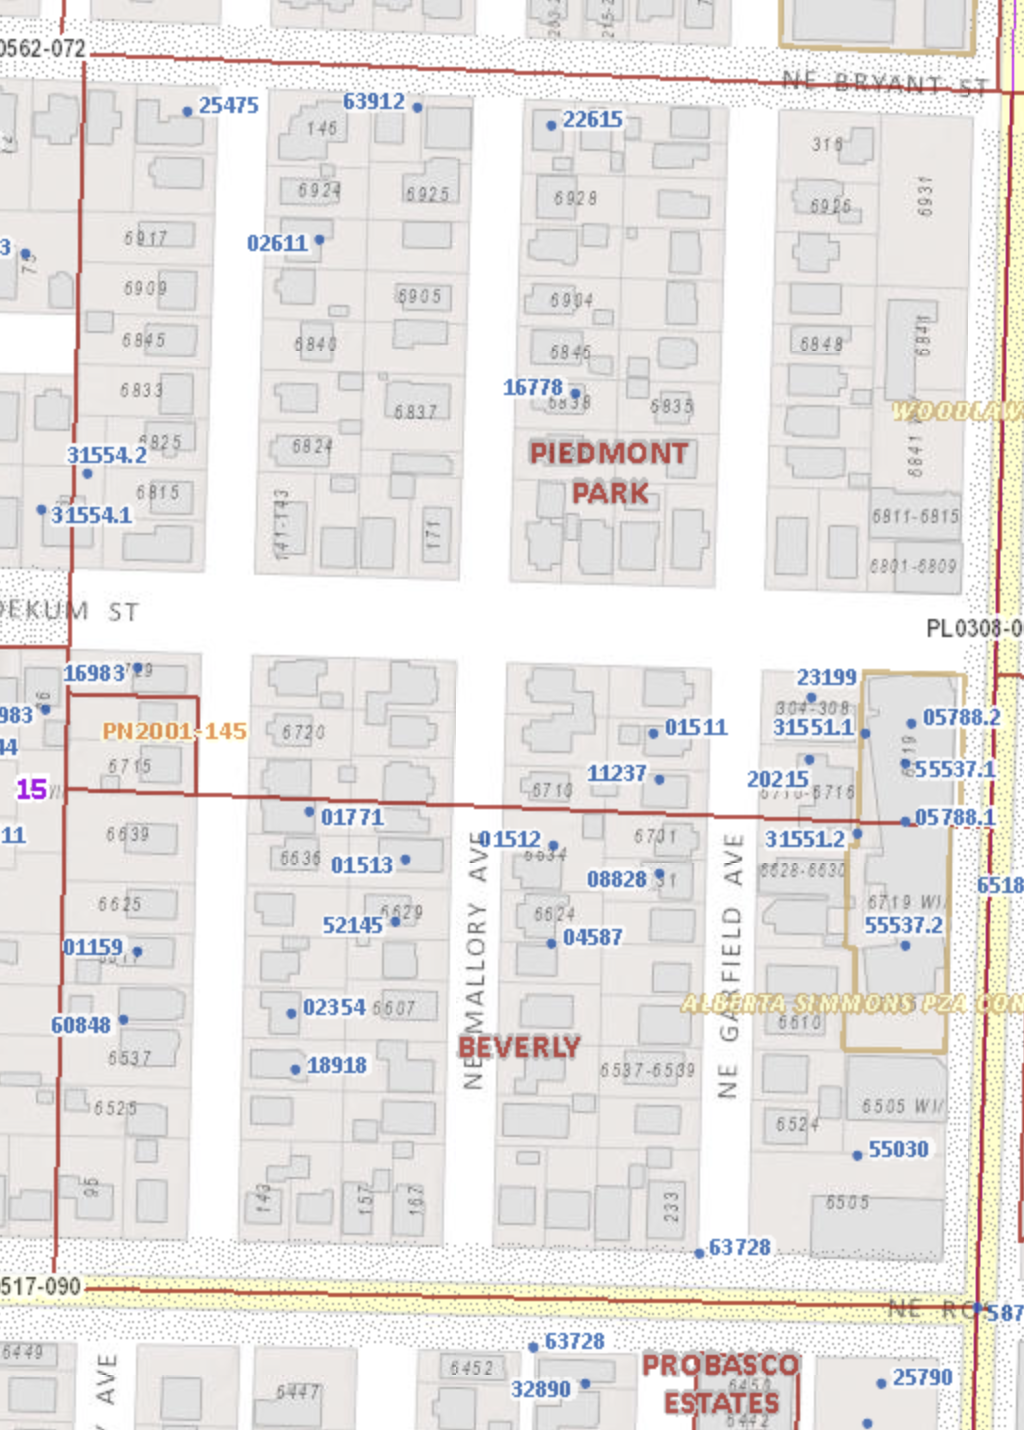
\includegraphics{images/image3.png}
\caption{alt\_text}
\end{figure}

The street names have not changed much since 1908, except for Pippin Street, which became Lombard Street in 1909. The full recorded plat document, with the text, is at

\url{https://drive.google.com/open?id=1DkSAk09dy4P8WEnhIk2DoUidFOkjt3ZD}

Houses

In a later part of this chapter I will look in detail at who built a house on the lot, and who lived in the house over the years. To get a global idea of 8 North Stafford Street and environs I use Sanborn map 459 for 1924-1928.

{\textgreater\textgreater\textgreater\textgreater\textgreater{} gd2md-html alert: inline image link here (to images/image4.png). Store image on your image server and adjust path/filename/extension if necessary. }(Back to top)(Next alert){\textgreater\textgreater\textgreater\textgreater\textgreater{} }

\begin{figure}
\centering
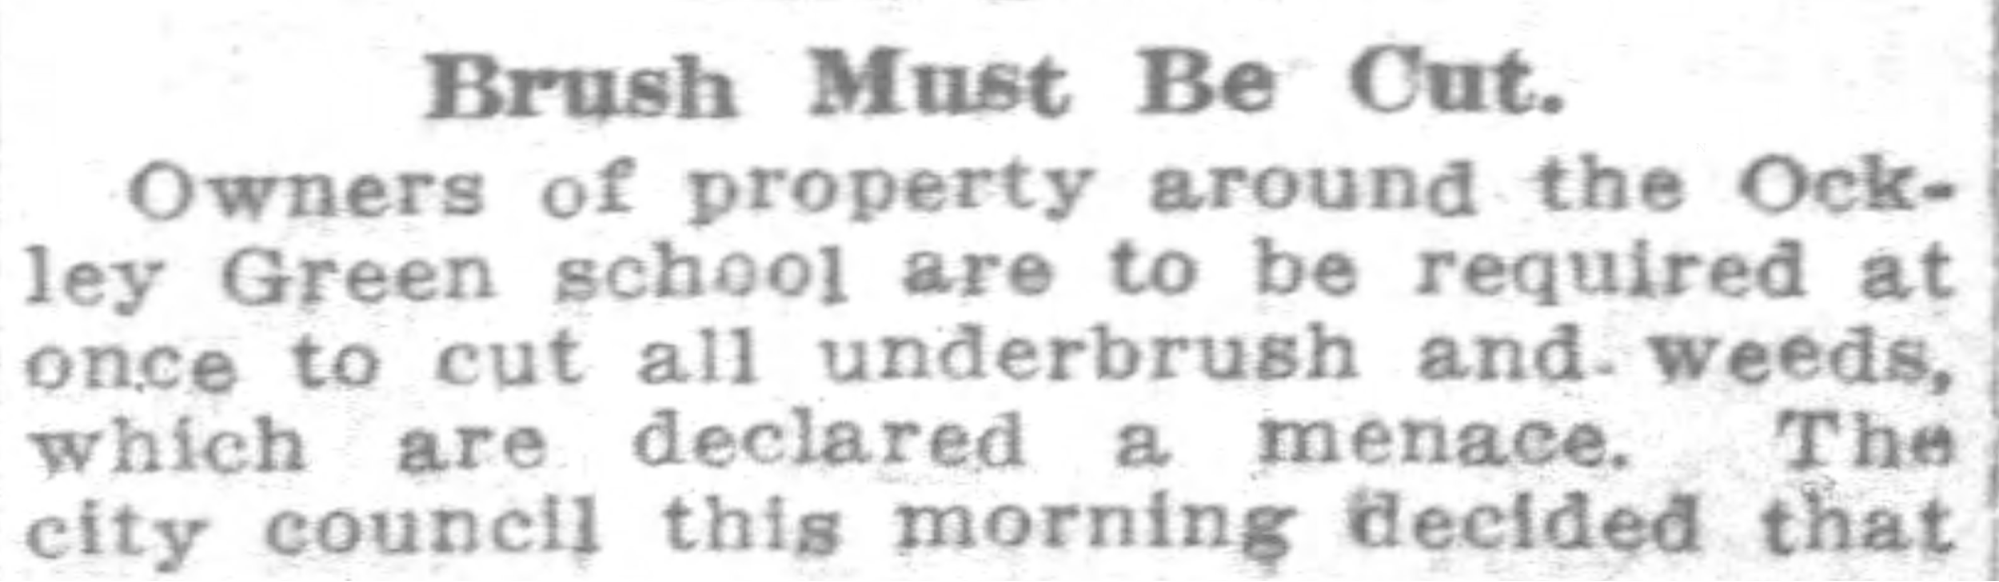
\includegraphics{images/image4.png}
\caption{alt\_text}
\end{figure}

It is unclear to me why Sanborn has both 1555 Williams and 1549 Williams on a single corner lot, because the plat map shows two lots, numbers 11 and 12. The Sanborn map shows our house as a frame house with a stone porch facing Williams at street number 1555. Much of block 6 of Loveleigh has not been built up yet, and in particular the neighboring lot 13 on Stafford is still empty.

In the next Sanborn map, which is not clearly dated but probably represents the situation around 1950, there now is an added garage on what used to be 1555 Williams, but became 7333 North Williams in the Great Renumbering of 1932. The map is kind enough to show both the old and the new number. There now is a house on what was 260 Stafford, which became 26 North Stafford. Some of the 100 by 100 feet corner lots that were unpartitioned in 1924-1928 are now split into two lots, corresponding to the original plat map. The house on lot 12 still has a porch facing Williams, which is of interest, because sometime in the 1950's the address changed to 8 North Stafford Street and the porch moved to the north side of the house. We will find out more about this change later.

{\textgreater\textgreater\textgreater\textgreater\textgreater{} gd2md-html alert: inline image link here (to images/image5.png). Store image on your image server and adjust path/filename/extension if necessary. }(Back to top)(Next alert){\textgreater\textgreater\textgreater\textgreater\textgreater{} }

\begin{figure}
\centering
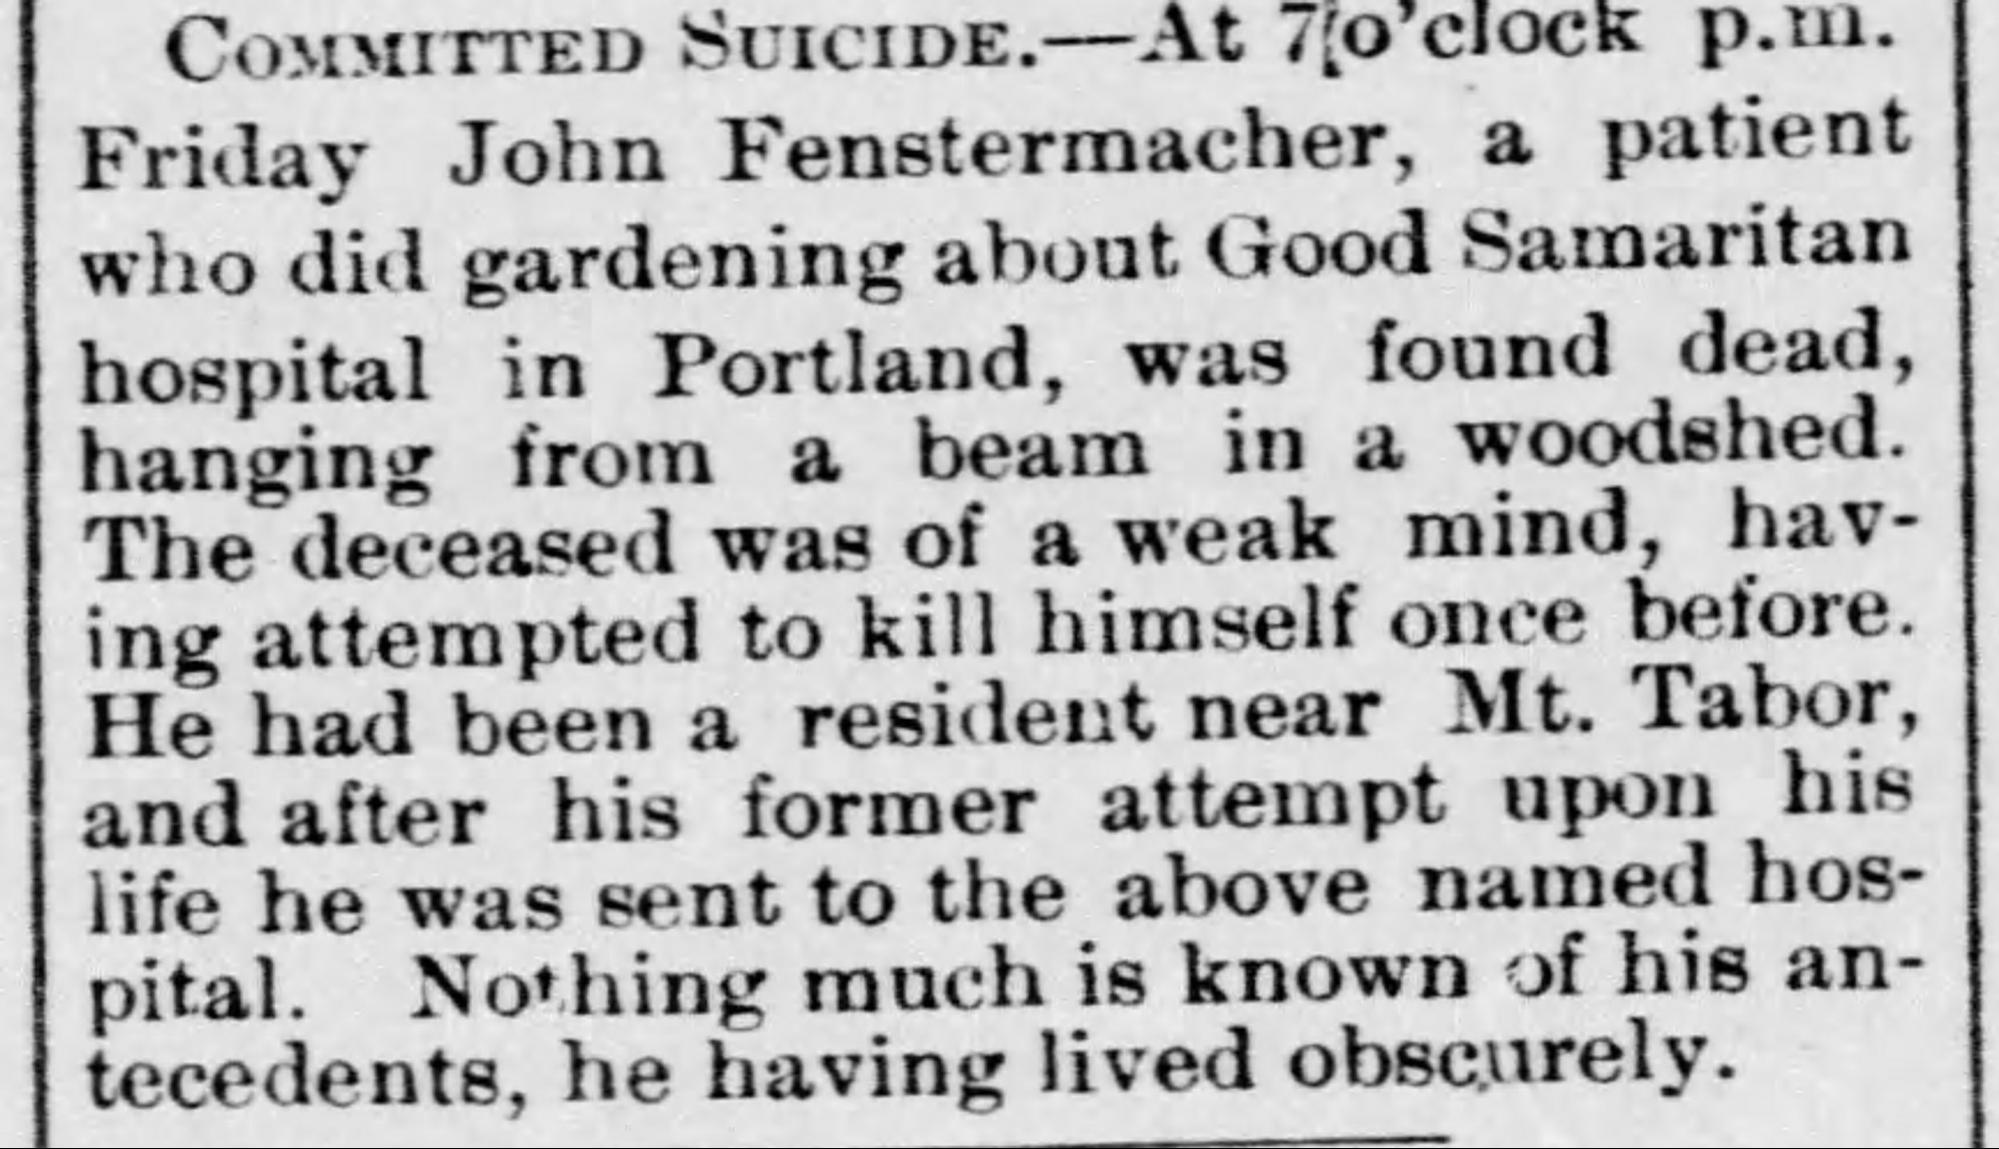
\includegraphics{images/image5.png}
\caption{alt\_text}
\end{figure}

Owners

In this section I trace the ownership of the property, which means the land plus the house, over the years. Every time the property changes hands, I include a link to the deed. In some cases I have some additional information about the owners, and I include that as well. I will start right after Loveleigh was platted.

The Brong Company

Since 1908 block 6, lot 12, of Loveleigh was owned by the Brong Company. The Oregonian of February 13, 1917 shows that in 1915 they still owed it, because they owed delinquent taxes on the property.

{\textgreater\textgreater\textgreater\textgreater\textgreater{} gd2md-html alert: inline image link here (to images/image6.png). Store image on your image server and adjust path/filename/extension if necessary. }(Back to top)(Next alert){\textgreater\textgreater\textgreater\textgreater\textgreater{} }

\begin{figure}
\centering
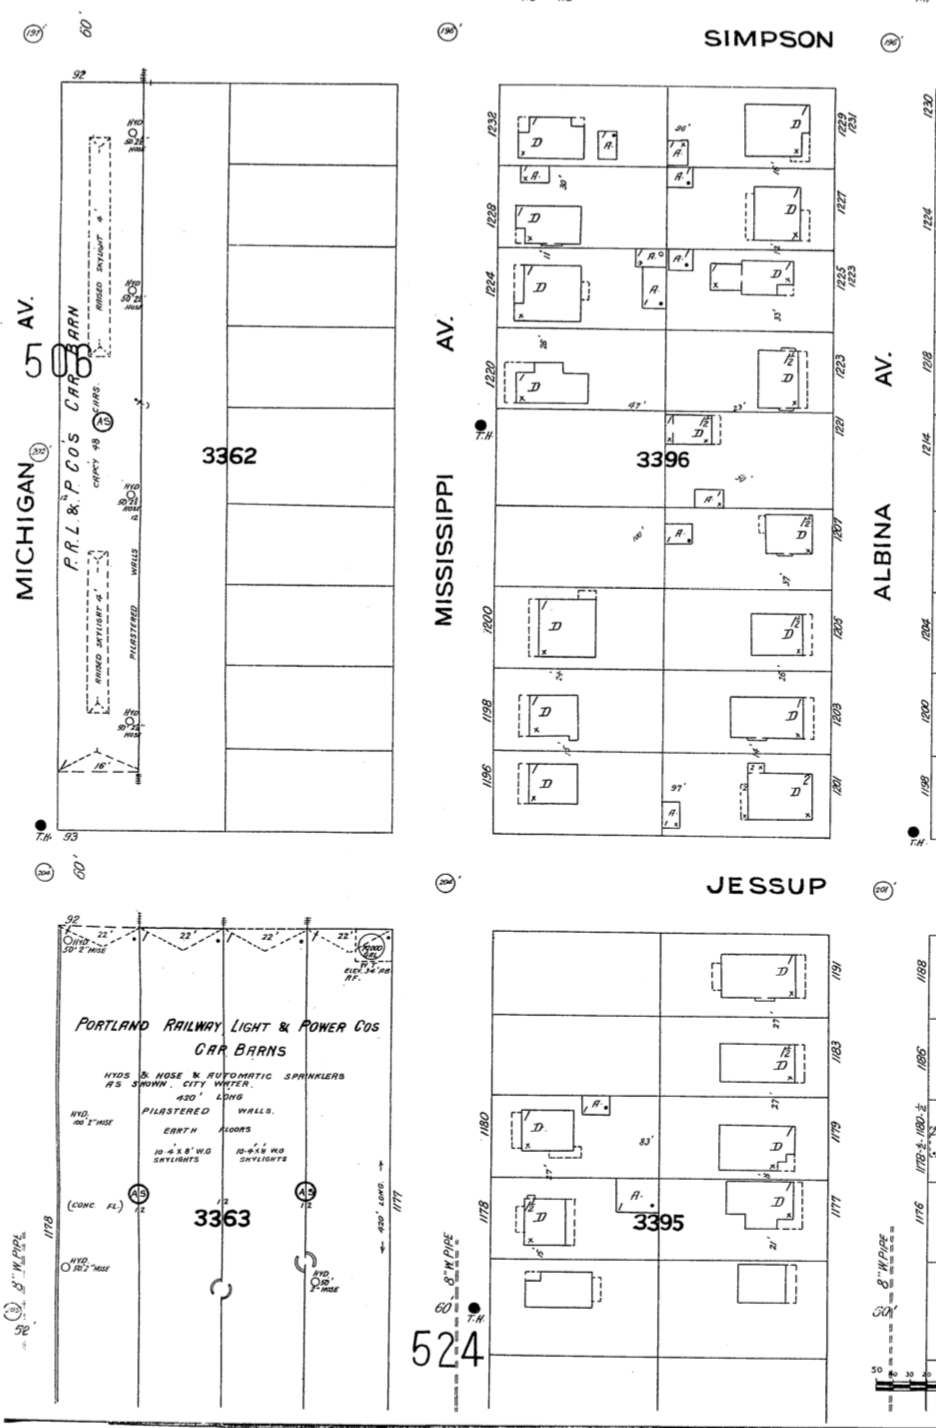
\includegraphics{images/image6.png}
\caption{alt\_text}
\end{figure}

There was no house on the lot for quite a long time, but things started moving around 1920.

Carrie Johnson and Peter Johnson

On February 24, 1920 the Brong Company sold the lot to Peter Johnson for \$ 650. The deed has the following binding provisions.

{\textgreater\textgreater\textgreater\textgreater\textgreater{} gd2md-html alert: inline image link here (to images/image7.png). Store image on your image server and adjust path/filename/extension if necessary. }(Back to top)(Next alert){\textgreater\textgreater\textgreater\textgreater\textgreater{} }

\begin{figure}
\centering
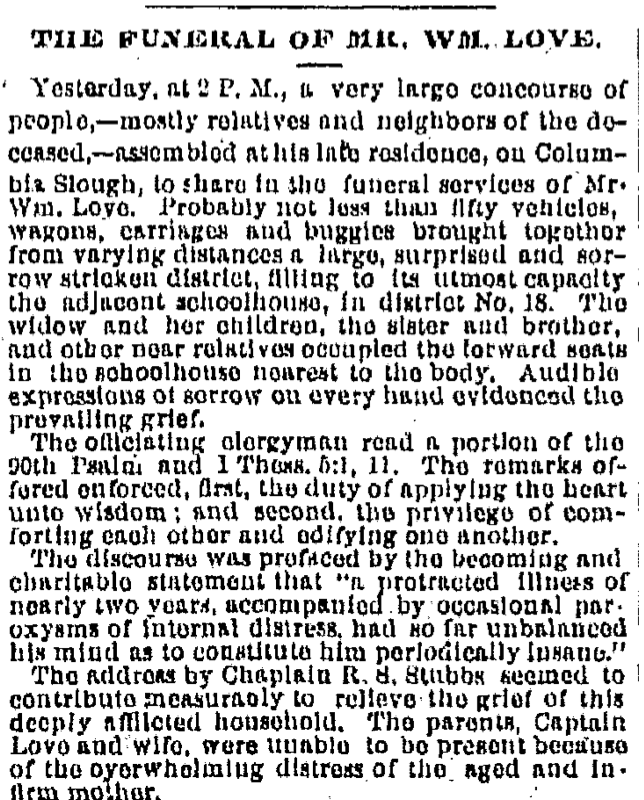
\includegraphics{images/image7.png}
\caption{alt\_text}
\end{figure}

\url{https://drive.google.com/open?id=1JgZZP86JOW5jR7oKp9PPsTf1l6AtYoX5}

Katie M. Merrifield and N. W. Merrifield

On March 17, 1920 Johnson, a month after buying it, transferred lot 12 in block 6 of Loveleight to N. W. Merrifield, a Vancouver real estate dealer specializing in rural acreage. The deed tells us Merrifield paid \$ 500 for the lot, a loss of \$ 150. The provisions imposed by the Brong Company were still in effect.

\url{https://drive.google.com/open?id=1lQWA6MlP-JCGsnw0x5rTwraOBp44DNFu}

I think we can safely assume that neither Johnson nor Merrifield ever lived on the lot, because of the short time they owned it, and because there was no house there yet. I am not sure what their deal was.

Alma Radditz and Francis M. Radditz

On April 7, 1921 Merrifield sold to Alma and Francis M. Radditz. Here is the deed.

\url{https://drive.google.com/open?id=1Z5F0jLqCHmnl9N4zTOnaHkYAL2505EeA}

And here is the building permits section of the Oregon Daily Journal of April 30, 1921.

{\textgreater\textgreater\textgreater\textgreater\textgreater{} gd2md-html alert: inline image link here (to images/image8.png). Store image on your image server and adjust path/filename/extension if necessary. }(Back to top)(Next alert){\textgreater\textgreater\textgreater\textgreater\textgreater{} }

\begin{figure}
\centering
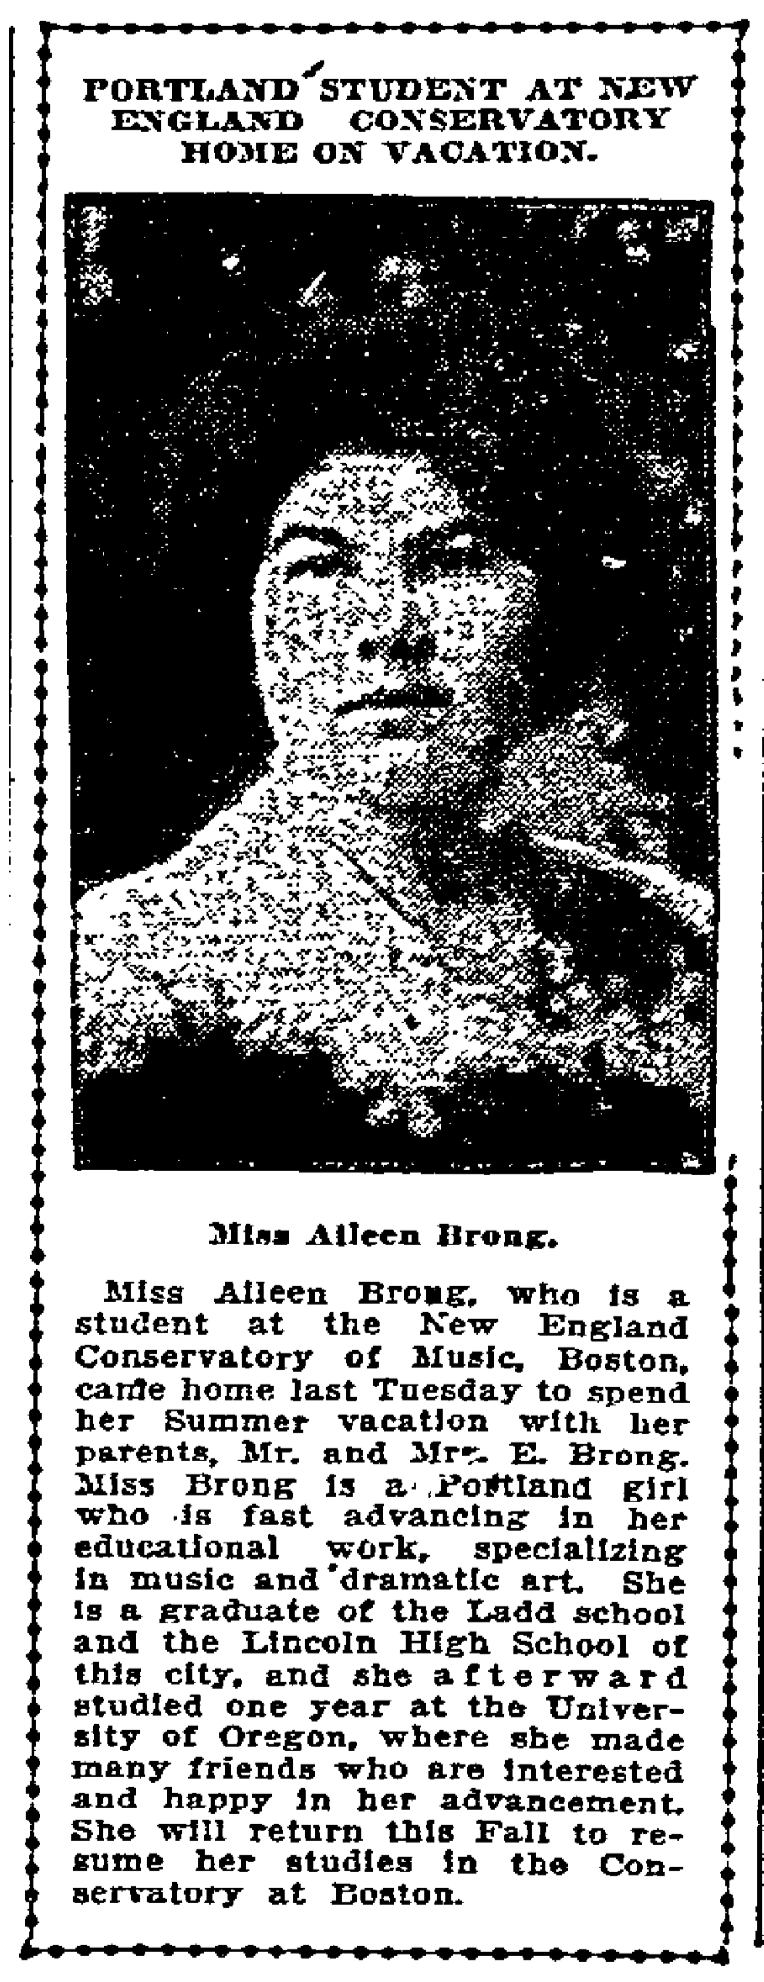
\includegraphics{images/image8.png}
\caption{alt\_text}
\end{figure}

We now know who built the house ! The cost of the building it was \$ 2,300, well over the \$ 1,000 limit specified by the Brong Company. No contractor was listed to do the building, which can mean that either the Radditzes did everything themselves, or that they bought a kit house. At that time kit houses, a.k.a. mail order houses, were very popular, and there were several companies in Portland that made them. Or they could be bought from companies such as Sears, who delivered the kit to the place where the house was to be assembled. As we shall see next, in the biography of Francis Radditz, he was a carpenter and welder, and thus probably quite capable of putting together a kit house.

Francis M. Radditz was born in 1895 or 1896 in Black Rock, Oregon. When the U.S. Army started recruiting in 1916-1917 for the impending war with Germany, Francis was sent to the recruiting station by Miss Ruby C. Price, postmistress of Black Rock. There he impressed the recruiters with his chest expansion. Here is an article from the Oregonian of February 25, 1917.

{\textgreater\textgreater\textgreater\textgreater\textgreater{} gd2md-html alert: inline image link here (to images/image9.png). Store image on your image server and adjust path/filename/extension if necessary. }(Back to top)(Next alert){\textgreater\textgreater\textgreater\textgreater\textgreater{} }

\begin{figure}
\centering
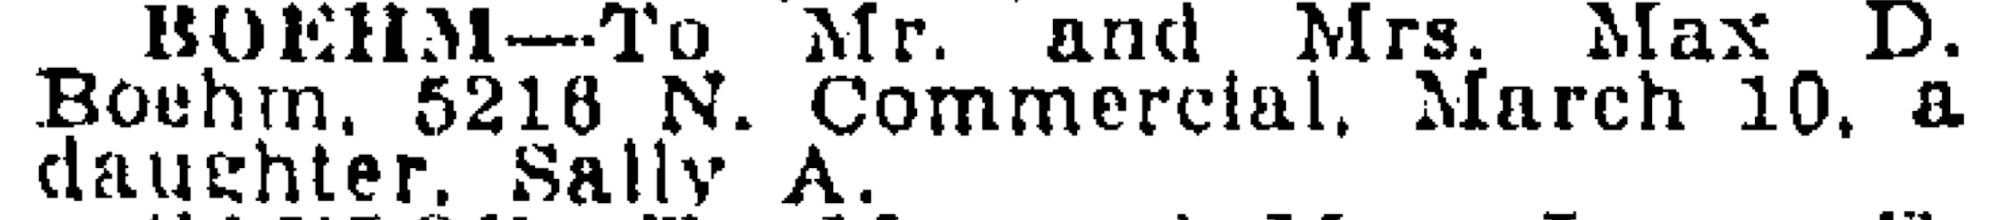
\includegraphics{images/image9.png}
\caption{alt\_text}
\end{figure}

Also on November 22, 1917 he married Alma Gottleib, from Hillsboro. On April 30, 1918 Sergeant Francis M. Radditz departed from Hoboken on U.S. Martha Washington to France, to serve on Company ``E'' Fourth Engineers, Fourth Division, Regular.

{\textgreater\textgreater\textgreater\textgreater\textgreater{} gd2md-html alert: inline image link here (to images/image10.jpg). Store image on your image server and adjust path/filename/extension if necessary. }(Back to top)(Next alert){\textgreater\textgreater\textgreater\textgreater\textgreater{} }

\begin{figure}
\centering
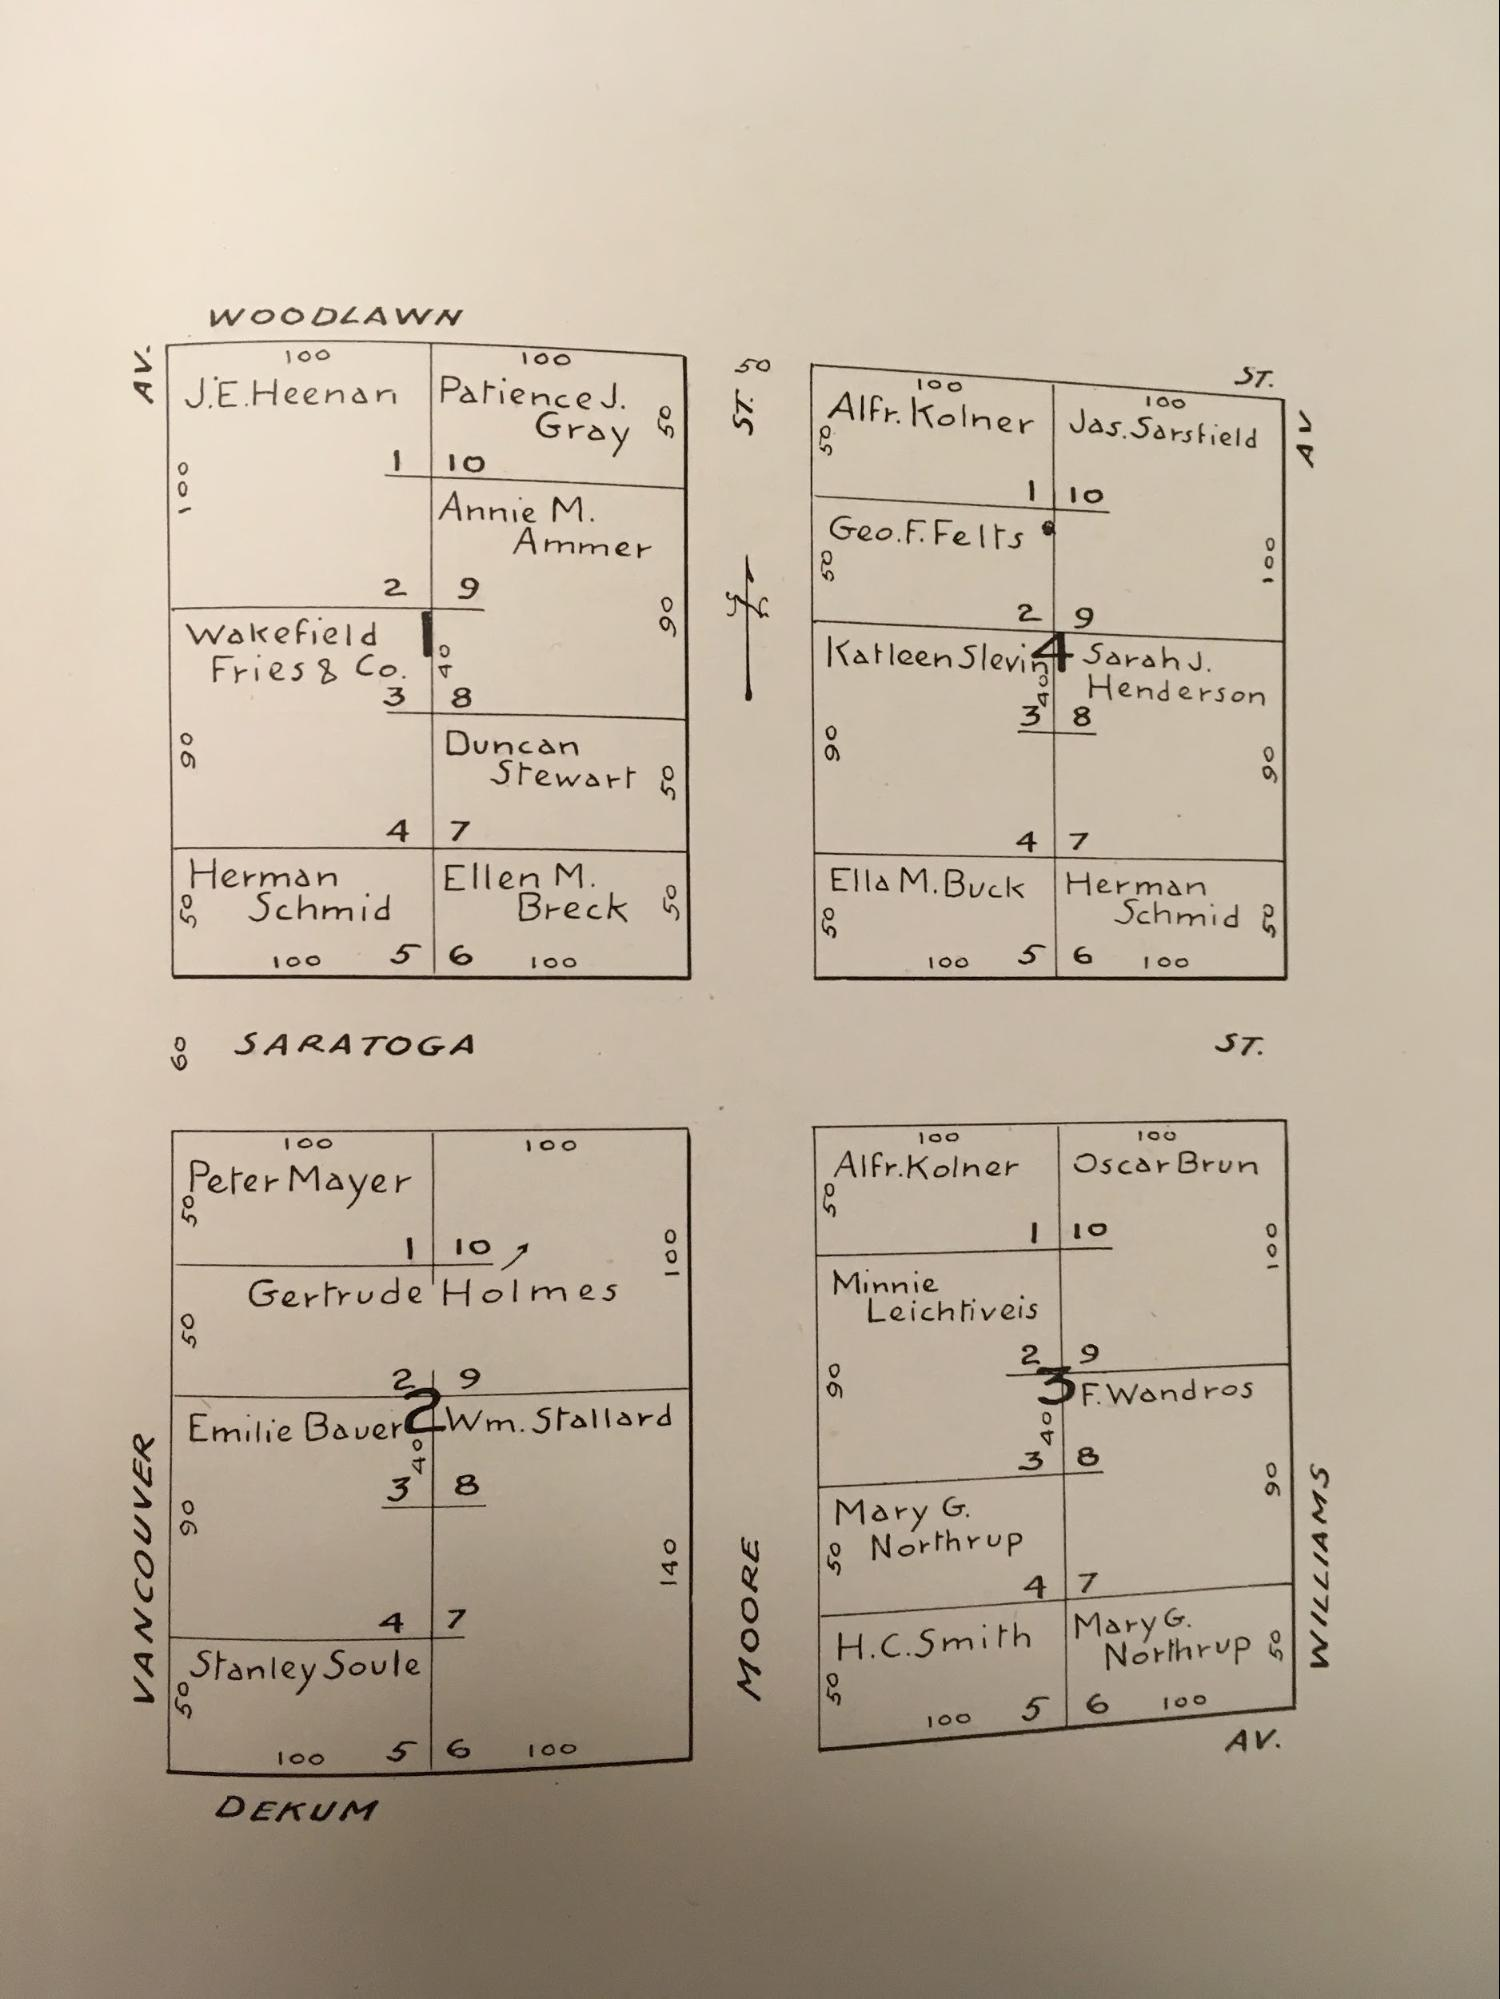
\includegraphics{images/image10.jpg}
\caption{alt\_text}
\end{figure}

On July 21, 1919 he was on his way back from Brest, on the U.S. Von Steuben, arriving at Hoboken on July 29.

{\textgreater\textgreater\textgreater\textgreater\textgreater{} gd2md-html alert: inline image link here (to images/image11.jpg). Store image on your image server and adjust path/filename/extension if necessary. }(Back to top)(Next alert){\textgreater\textgreater\textgreater\textgreater\textgreater{} }

\begin{figure}
\centering
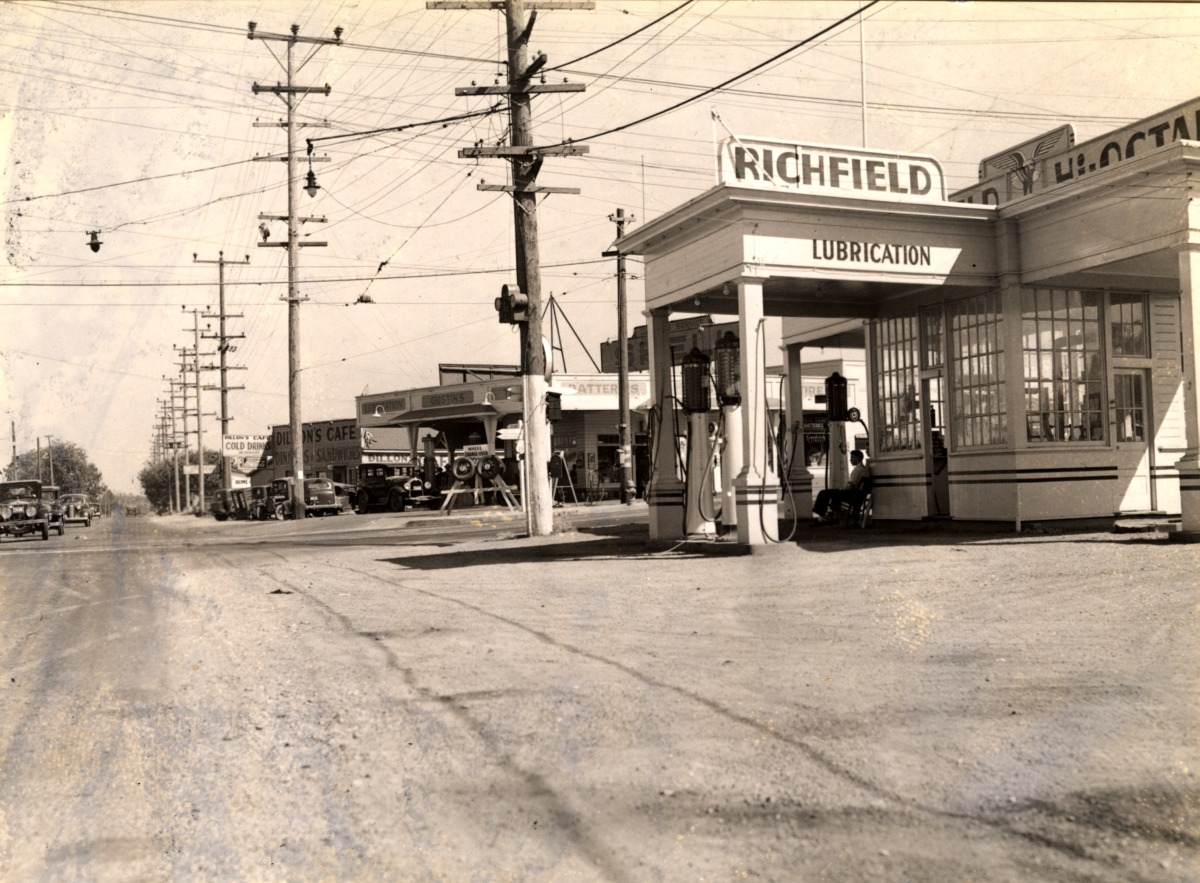
\includegraphics{images/image11.jpg}
\caption{alt\_text}
\end{figure}

Newspaper articles list him as one of the Oregonians who was ``slightly wounded'' during the war. In the meantime Alma had given birth to Francis M. Radditz Jr.~on January 21, 1919.

The Radditz family seemed to have moved around before they settled at 1555 Williams Avenue. When Francis went to war in 1918 they lived at 507 East Seventh Street in Vancouver. Junior was born in 1919 at 414 Eleventh Street in Portland. At the 1920 census Alma and Francis M. Junior lived on the farm of Alma's mother (widowed) on North Plains Road in Hillsboro. In 1921 the Vancouver City Directory has the family at 2014 C Street. Alma was clerk at the confectionery shop of Matthias O. Spurgeon, who incidentally was granted U.S. patent No 1,111,870 in 1914 for a marshmallow toasting machine. At that time, Francis was a welder at the G. M. Standiver Corporation, shipbuilders in Vancouver.

Then, in the same year 1921, the Portland City Directory has the family residing at 1555 Williams, in what is now our house, with Francis a self-employed carpenter. As we will see further on, the Radditzes sold that house in 1924 to the Reed family. In 1925 Alma contracted with Dwight Cheney to build a house at 843 East Sixteenth Street North for \$ 4,500, and in the 1930 census we see the family there, with Francis again listed as a welder, working in ``the electric works''. At that last address, with the new street number, something went terribly wrong. See this clip from the Oregonian of August 7, 1934.

{\textgreater\textgreater\textgreater\textgreater\textgreater{} gd2md-html alert: inline image link here (to images/image12.png). Store image on your image server and adjust path/filename/extension if necessary. }(Back to top)(Next alert){\textgreater\textgreater\textgreater\textgreater\textgreater{} }

\begin{figure}
\centering
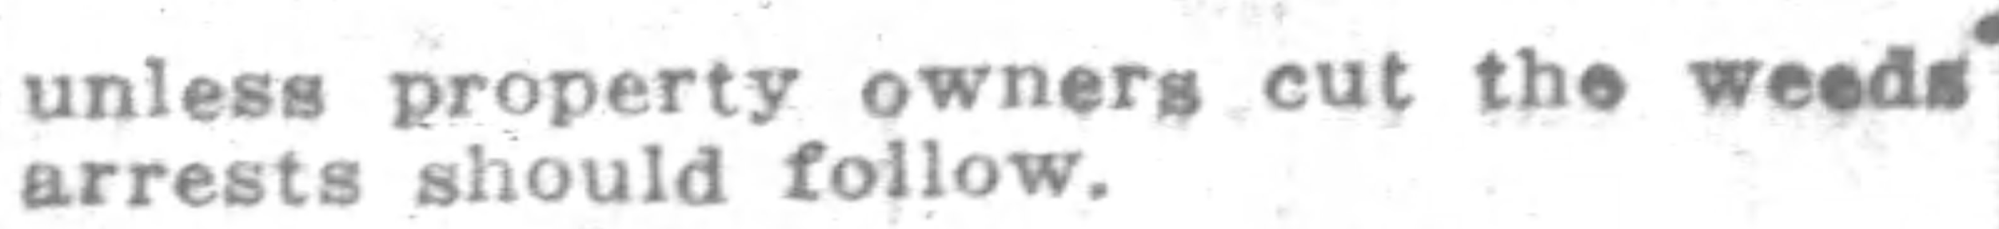
\includegraphics{images/image12.png}
\caption{alt\_text}
\end{figure}

Alma was buried in the Hillsboro Pioneer Cemetery. Francis Sr.~lived until 1972. Although the Radditz family lived on the corner of Williams and Stafford for only three years, they were the ones who built the house.

Anna D. Reed and Leonard J. Reed

On September 24, 1924 Alma and Francis M. Radditz sold the house at 1555 Williams Avenue to Anna D. and Leonard J. Reed. Here is the deed.

\url{https://drive.google.com/file/d/12UCjj03cyRnIO-IH4QWPjcy4ReJndgsB/view?usp=sharing}

The deed does not mention the actual sales price, only a nominal amount of \$ 10. It does say, however:

\begin{verbatim}
_That the above mentioned premises are free from all incumbrances except one certain mortgage of Fifteen Hundred Dollars which the grantees agree to assume and pay._
\end{verbatim}

Although the Radditz family built the house, and presumably lived in it for a while, the Reed family was the first family to live in the house for a substantial amount of time, in fact for about twenty years.

What do we know about them ? Leonard Joe Reed was born in Wade, Jasper County, Illinois in 1897. In the 1900 federal census he still lived there on the farm, with his parents William and Naomi and two sisters. In the 1910 census we find the family on a farm in Wind Mountain, Skamania, Washington. The 1920 census shows Leonard Joe and Anna Delilah Reed living with William and Naomi in Vancouver, Washington. William is now a retired farmer, with his own home, and Leonard is a machinist at a shipyard. Anna used to be Anna Davids, daughter of Frank Davids, also a farmer from Wind Mountain, Skamania, Washington. That must have been where they met. The census also shows the highest level of education both attained was eight grade. That must have been how they met. Leonard and Anna married in 1919.

{\textgreater\textgreater\textgreater\textgreater\textgreater{} gd2md-html alert: inline image link here (to images/image13.png). Store image on your image server and adjust path/filename/extension if necessary. }(Back to top)(Next alert){\textgreater\textgreater\textgreater\textgreater\textgreater{} }

\begin{figure}
\centering
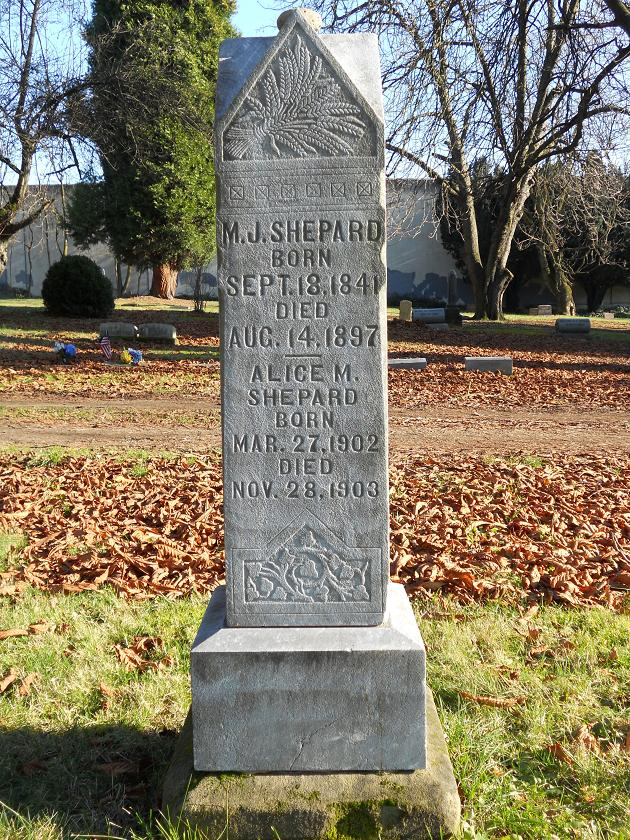
\includegraphics{images/image13.png}
\caption{alt\_text}
\end{figure}

There is some additional information on Leonard's first world war draft registration card of June 1918. It turns out that the shipyard in Vancouver where he worked was owned by G. M. Standivar, and that is the same shipyard where Francis M. Radditz was a welder at the time. Thus the two men may have known each other, and that may actually have been how Leonard knew about the house at 1555 Williams that Francis lived in and sold in 1924.

The same registration card shows that in 1918 Leonard lived on East Sixth Street N. The city directories show that in 1921 Leonard and Anna owned a home at 596 Union Avenue N. But then, finally, the 1930 census has Leonard and Anna living at 1555 Williams Avenue. They have a nine year old daughter named Genevieve. Leonard is foreman on a steam railroad, which the city directories reveal to be the Southern Pacific. The house is valued at \$ 3,600. The 1940 census shows Leonard as an inspector on that same steam railroad. Genevieve is now 19, and works as a stenographer in the insurance business, after finishing four years of high school. Although the Oregonian of May 31, 1939 tells us that on that day our house had the honor of hosting a true sorority group.

{\textgreater\textgreater\textgreater\textgreater\textgreater{} gd2md-html alert: inline image link here (to images/image14.png). Store image on your image server and adjust path/filename/extension if necessary. }(Back to top)(Next alert){\textgreater\textgreater\textgreater\textgreater\textgreater{} }

\begin{figure}
\centering
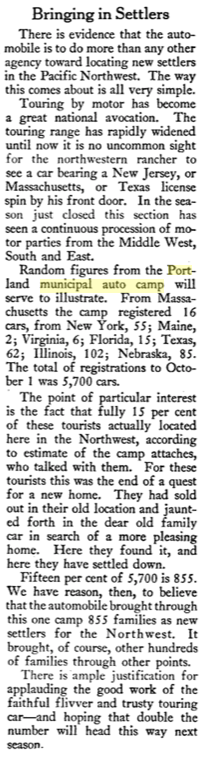
\includegraphics{images/image14.png}
\caption{alt\_text}
\end{figure}

Genevieve, who seems to have been an only child, married in 1941, and moved out of the house (and maybe dropped out of college). I have a picture from a high school yearbook, but unfortunately I do not remember where I found it. At least I hope it is her.

{\textgreater\textgreater\textgreater\textgreater\textgreater{} gd2md-html alert: inline image link here (to images/image15.png). Store image on your image server and adjust path/filename/extension if necessary. }(Back to top)(Next alert){\textgreater\textgreater\textgreater\textgreater\textgreater{} }

\begin{figure}
\centering
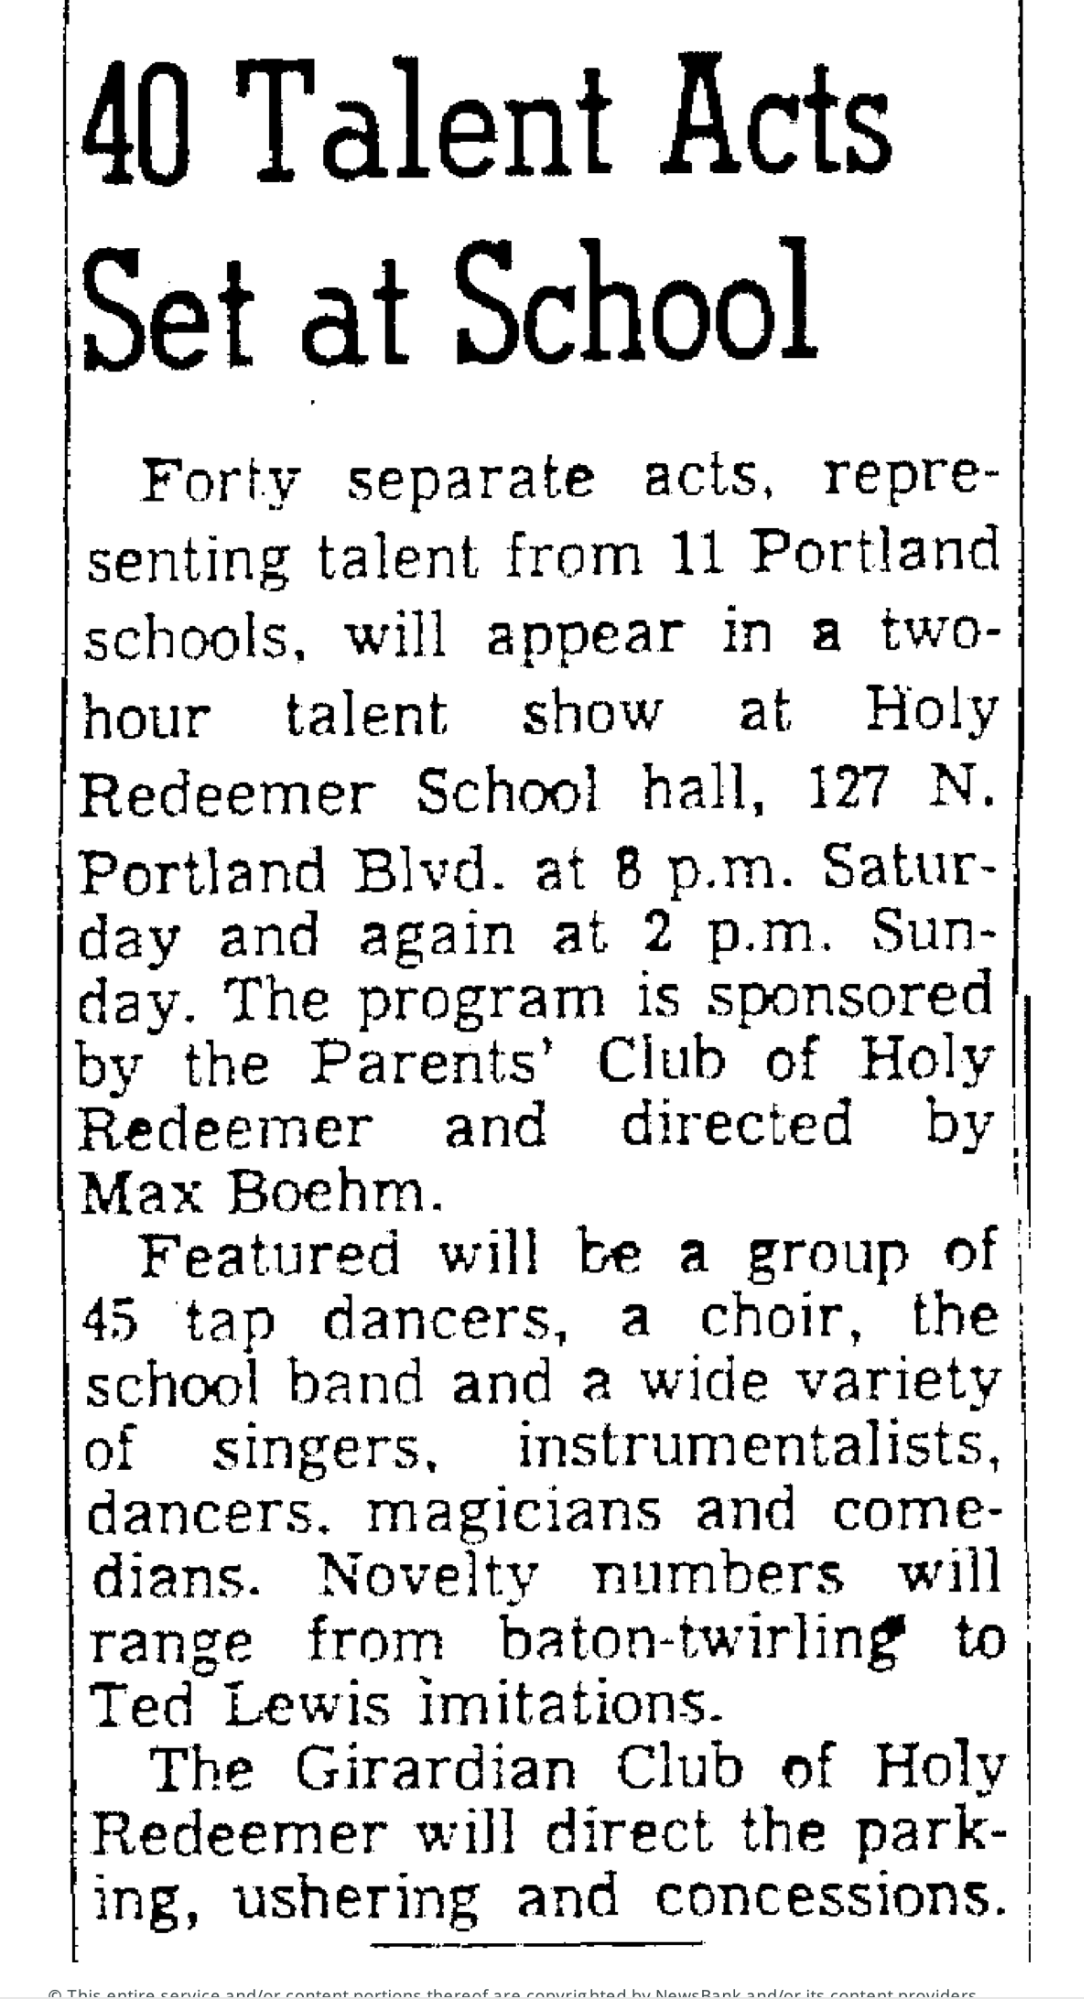
\includegraphics{images/image15.png}
\caption{alt\_text}
\end{figure}

{\textgreater\textgreater\textgreater\textgreater\textgreater{} gd2md-html alert: inline image link here (to images/image16.png). Store image on your image server and adjust path/filename/extension if necessary. }(Back to top)(Next alert){\textgreater\textgreater\textgreater\textgreater\textgreater{} }

\begin{figure}
\centering
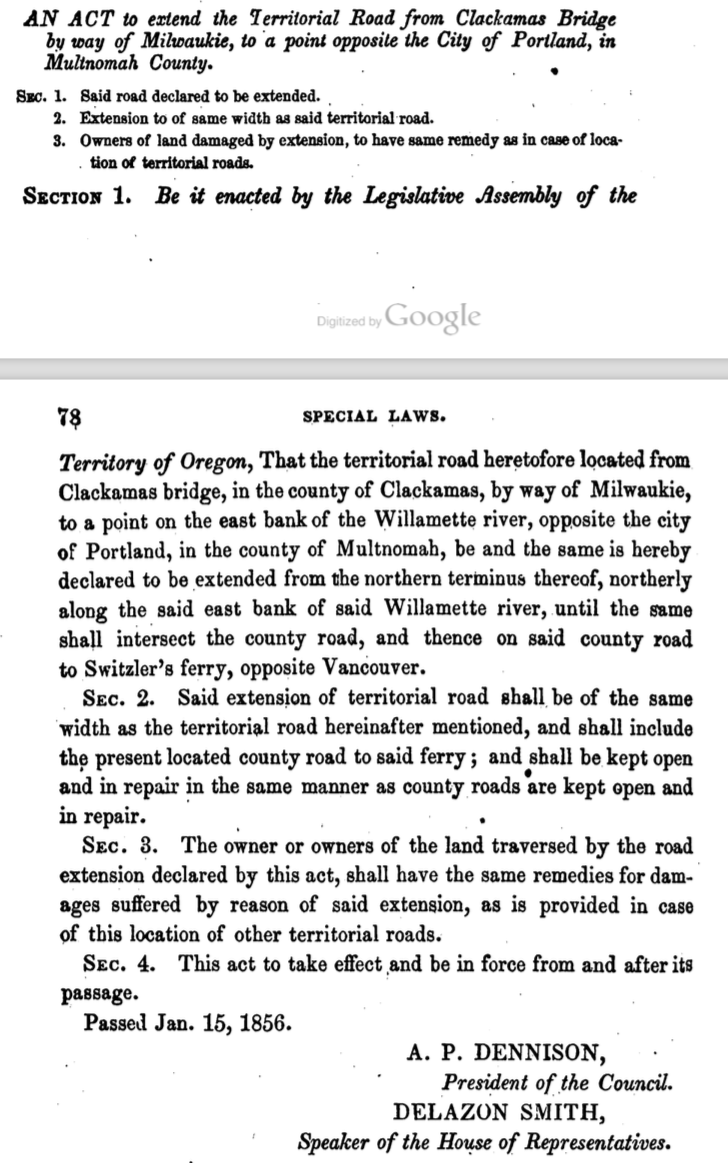
\includegraphics{images/image16.png}
\caption{alt\_text}
\end{figure}

Marjorie A. Gerhard and Harold C. Gerhard

Leonard and Anna sold the house on December 18, 1944 to Harold C. and Marjorie A. Gerhard. I don't know where the Reeds moved to, but I do know that Leonard lived until 1952 and Anna until 1992.

The warranty deed of the sale to the Gerhards again gives a nominal amount of \$ 10 for the consideration. There are no encumbrances, except for 6 months of property taxes.

\url{https://drive.google.com/file/d/1PRS84Eid4wQab7zhpmxs-ElK481WjC7E}

We can be very brief on the Gerhards, because I am not even sure if they ever lived at what was now 7333 Williams Avenue. If they did, it was only for a brief period, because they sold it less than a year after buying it to Ben D. and Hulda H. Graf. In 1940 the Gerhards lived in Gardiner, in Douglas County, Oregon, at the mouth of the Umpqua River. They were very active socially, and Harold was elected to prominent positions in the local Lions Club and Odd Fellows Lodge. They sold their confectionary business and moved north in December 1944, which was when they bought the house on 7333 Williams. In the Roseburg News Review of December 11, 1944 we read about the move.

{\textgreater\textgreater\textgreater\textgreater\textgreater{} gd2md-html alert: inline image link here (to images/image17.png). Store image on your image server and adjust path/filename/extension if necessary. }(Back to top)(Next alert){\textgreater\textgreater\textgreater\textgreater\textgreater{} }

\begin{figure}
\centering
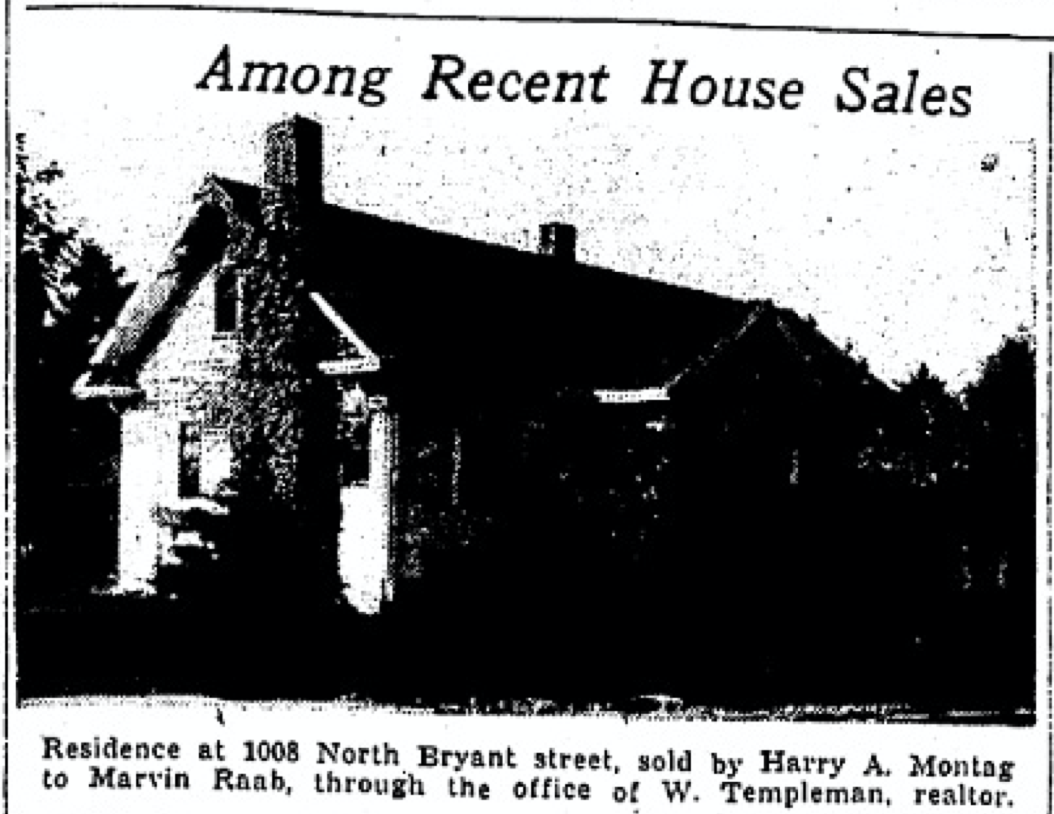
\includegraphics{images/image17.png}
\caption{alt\_text}
\end{figure}

But already in 1946 the Gerhards lived in Astoria, so it is unclear if they ever really stopped over in Portland.

Hulda H. Graf and Benjamin D. Graf

The next set of buyers, Benjamin Dwight and Hulda Hanna Graf, were even less likely to actually move into the house. They bought the house on November 14, 1945. Benjamin was born in 1888 in Bethany, which is now part of the greater Portland area, between Hillsboro and Forest Park. He married Hulda Hanna Scheel in 1918. He lived on his own farm all his working life, and he was already 56 when he bought 7333 Williams Avenue from the Gerhards. So it is likely he bought the place for investment. The deed does not specify the price, only the annoying \$ 10. There is no census document or city directory that shows him living in the house.

\url{https://drive.google.com/open?id=1Zx23hONVBnZL6A0wEJhLKfQEkEXfKuMp}

Marguerite E. Boehm and Max D. Boehm

The Grafs sold the property on August 10, 1949 to Max Dorwin Boehm and Marguerite Evelyn Boehm, again for an undisclosed price. Here is the deed.

\url{https://drive.google.com/open?id=1JUldb3Fv7rNkw-FJRHSopklS20TaJ1Gh}

The Boehms lived in the house for 22 years, until 1971. This makes them the second family who really made it their home. Max was born in 1918, and Marguerite Clark in 1916. They married in 1942.

{\textgreater\textgreater\textgreater\textgreater\textgreater{} gd2md-html alert: inline image link here (to images/image18.png). Store image on your image server and adjust path/filename/extension if necessary. }(Back to top)(Next alert){\textgreater\textgreater\textgreater\textgreater\textgreater{} }

\begin{figure}
\centering
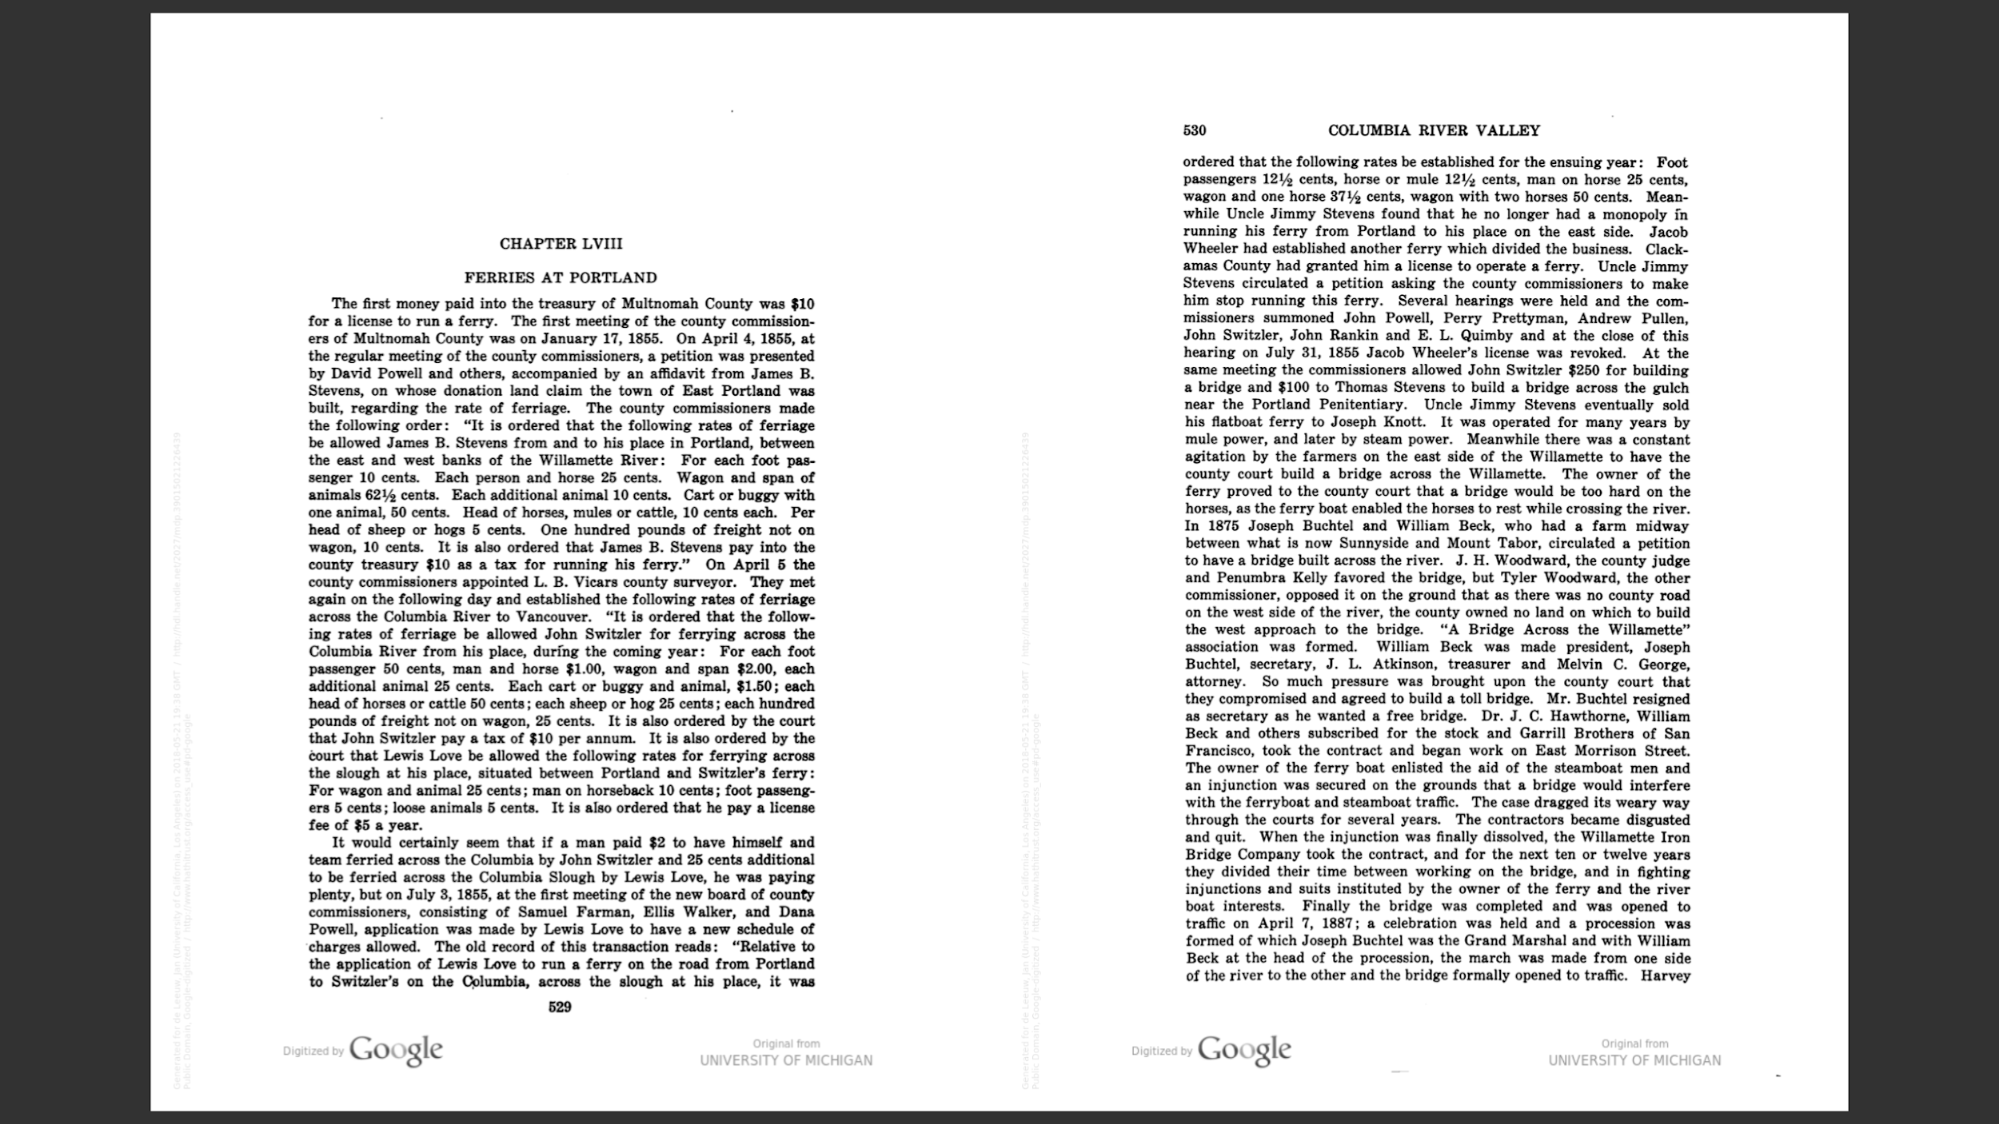
\includegraphics{images/image18.png}
\caption{alt\_text}
\end{figure}

Their first daughter Bonnie was born in 1943.

{\textgreater\textgreater\textgreater\textgreater\textgreater{} gd2md-html alert: inline image link here (to images/image19.png). Store image on your image server and adjust path/filename/extension if necessary. }(Back to top)(Next alert){\textgreater\textgreater\textgreater\textgreater\textgreater{} }

\begin{figure}
\centering
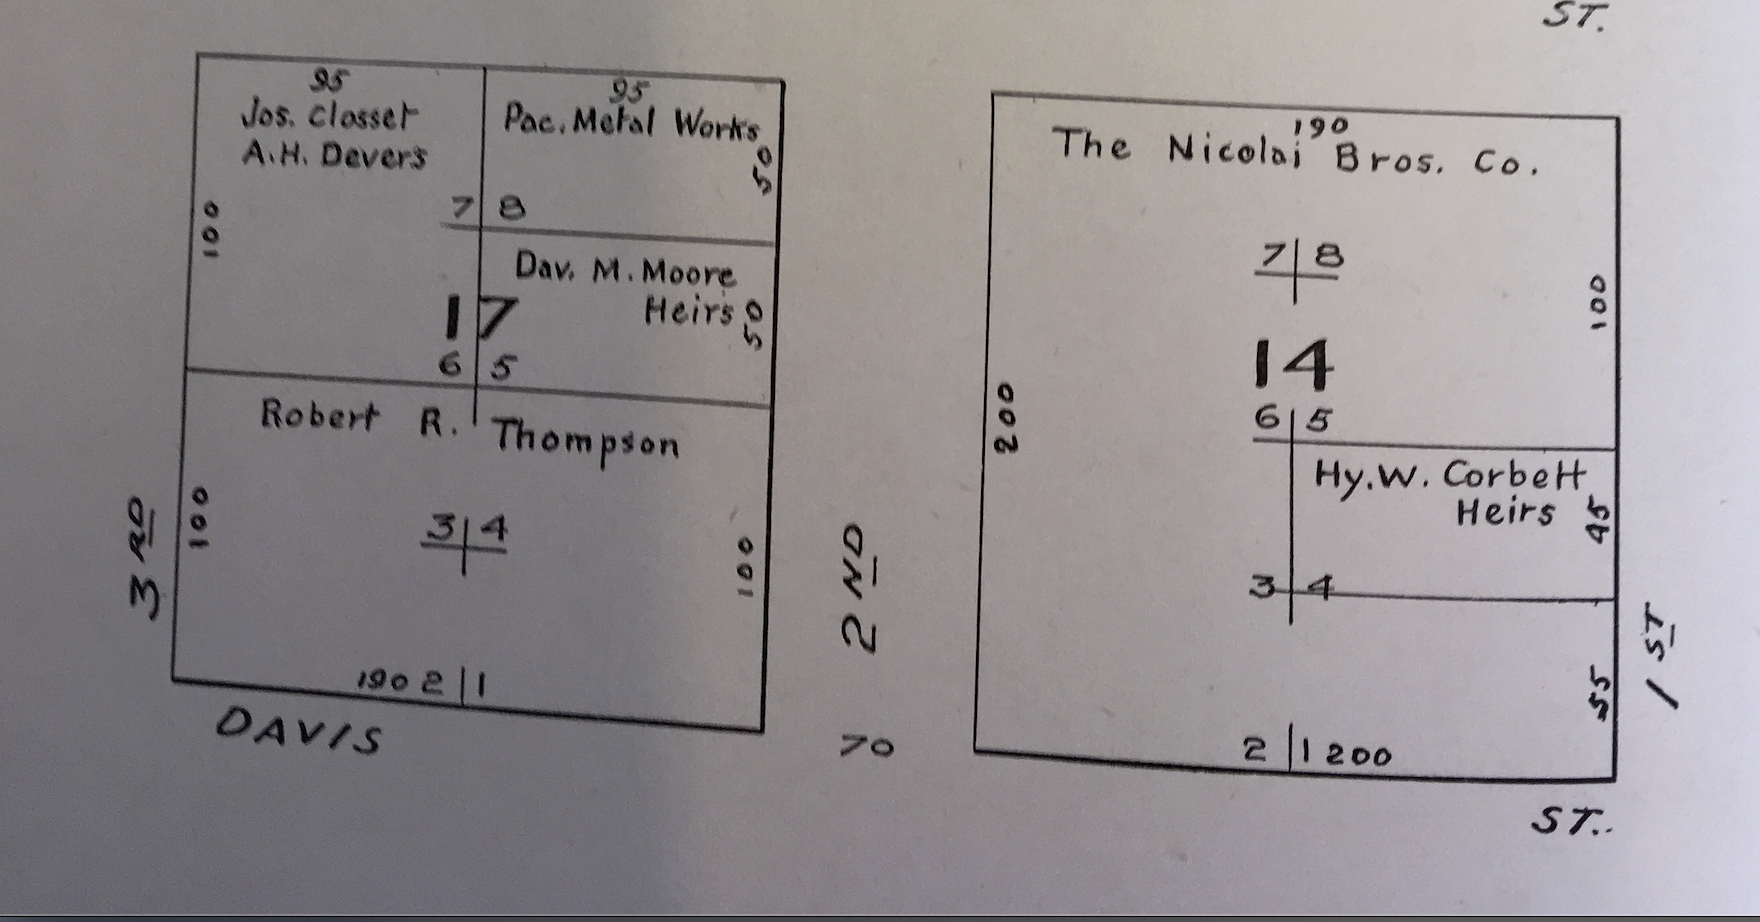
\includegraphics{images/image19.png}
\caption{alt\_text}
\end{figure}

The second daughter Sally was born in 1946.

{\textgreater\textgreater\textgreater\textgreater\textgreater{} gd2md-html alert: inline image link here (to images/image20.png). Store image on your image server and adjust path/filename/extension if necessary. }(Back to top)(Next alert){\textgreater\textgreater\textgreater\textgreater\textgreater{} }

\begin{figure}
\centering
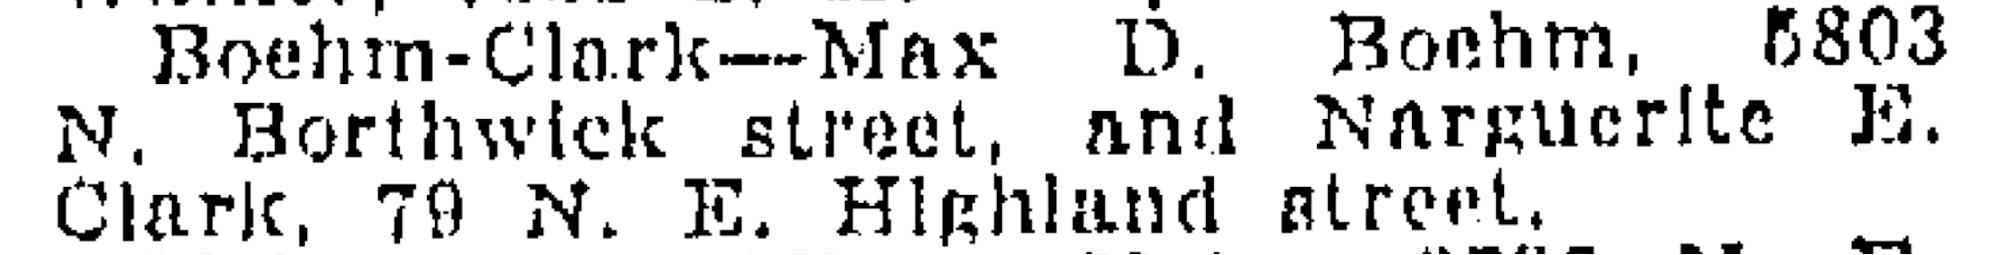
\includegraphics{images/image20.png}
\caption{alt\_text}
\end{figure}

As far as I can tell there were no more children, and the family was complete when they moved from Commercial to the Williams home.

From the city directories we get some idea about the kind of work Max did. In 1953, he was a solicitor (i.e.~a canvasser) for the National Carloading Corporation, a freight forwarding company. Its business was to collect, consolidate, ship freights which were less than a (railroad) carload. It employed the services of various carriers by motor vehicle and rail, and paid regular tariff rates to such carriers. Max was duly promoted over the years, and in the Oregonian of February 20, 1961 we see

{\textgreater\textgreater\textgreater\textgreater\textgreater{} gd2md-html alert: inline image link here (to images/image21.png). Store image on your image server and adjust path/filename/extension if necessary. }(Back to top)(Next alert){\textgreater\textgreater\textgreater\textgreater\textgreater{} }

\begin{figure}
\centering
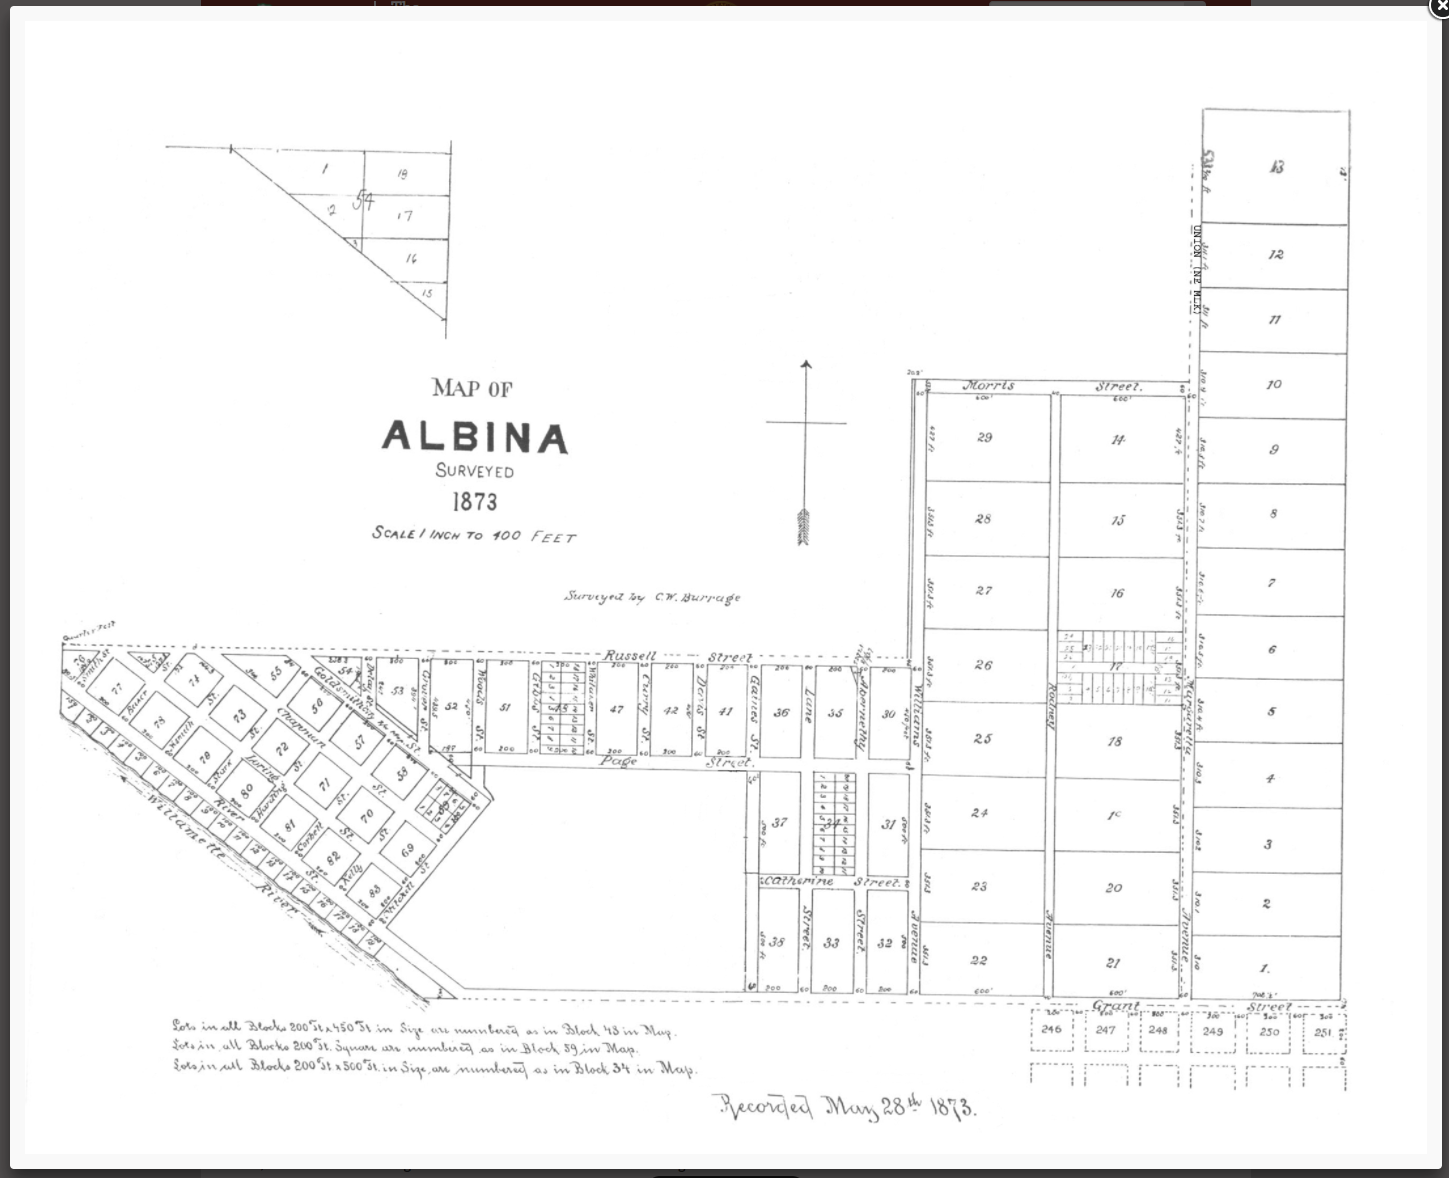
\includegraphics{images/image21.png}
\caption{alt\_text}
\end{figure}

But Max Boehm was also engaged in more artistic activities. Already in 1934, as a senior at Jefferson High, he acted in the play ``The Birthday of the Infanta'' at the freshman reception festivities. In 1957 the Portland PTA's organized Dad's Nights. At Clinton Kelly School

{\textgreater\textgreater\textgreater\textgreater\textgreater{} gd2md-html alert: inline image link here (to images/image22.png). Store image on your image server and adjust path/filename/extension if necessary. }(Back to top)(Next alert){\textgreater\textgreater\textgreater\textgreater\textgreater{} }

\begin{figure}
\centering
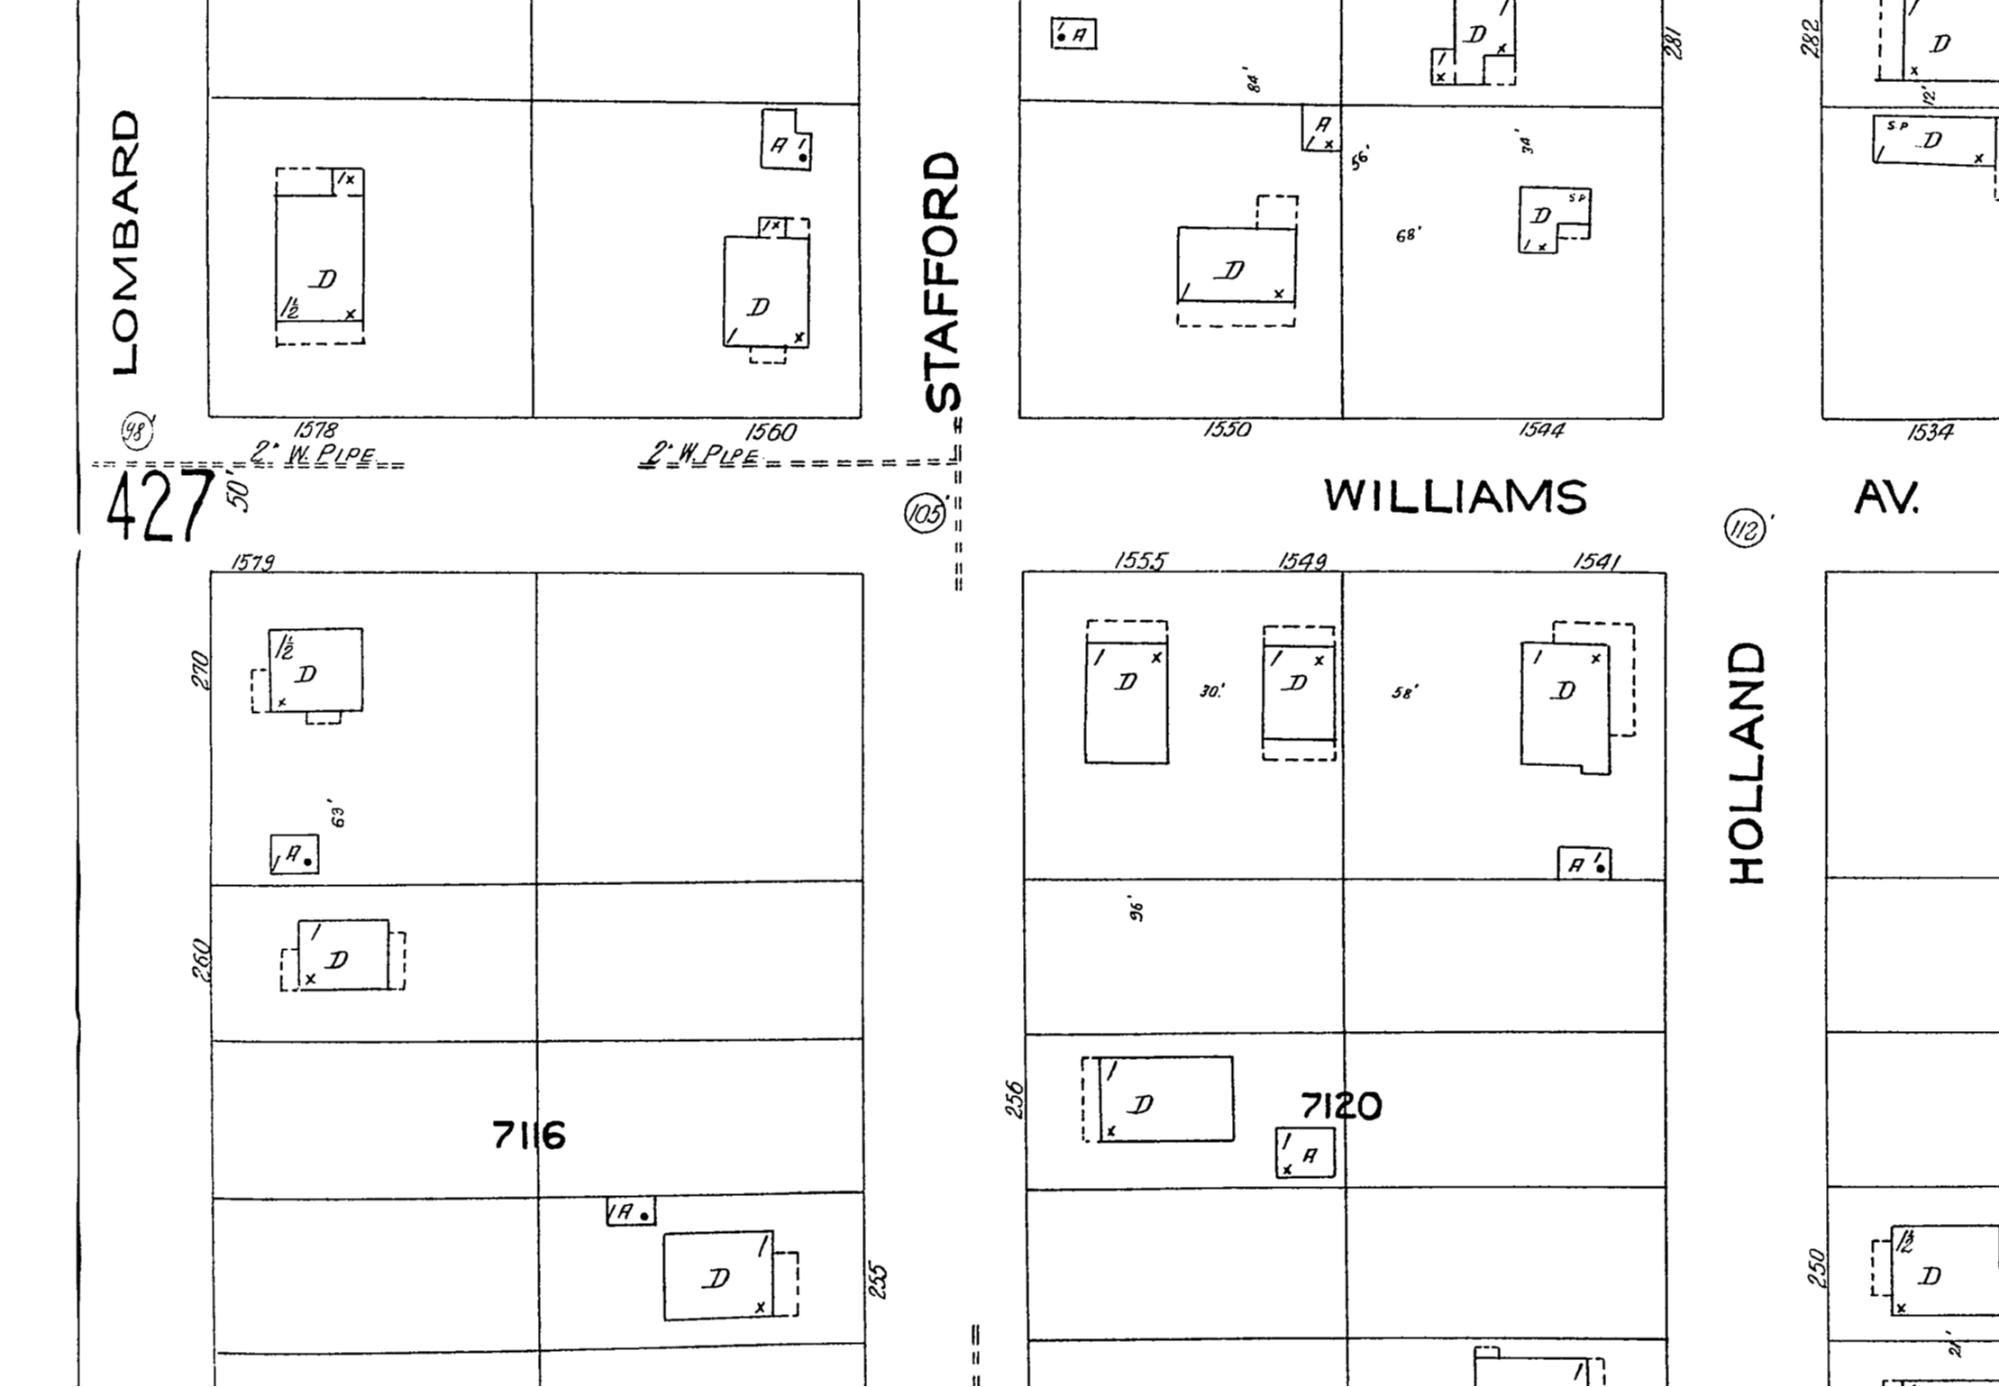
\includegraphics{images/image22.png}
\caption{alt\_text}
\end{figure}

In 2017, Nik and I were visited by the two Boehm daughters Bonnie and Sally, who were visiting their cousin Julie Clark, a neighbor on Stafford, across the street. On a little nostalgia tour we showed them what we had changed in the house, and they told us how it looked in the sixties and seventies, what had changed and what was still the same. They told us about tap dancing rehearsals in the basement, and about the change of the address from Williams Avenue to Stafford Street.

There were various attempts in the sixties by Marguerite and Max to sell the house, mostly by owner. I will document them with little advertisements from the Oregonian, because they have some interesting details.

{\textgreater\textgreater\textgreater\textgreater\textgreater{} gd2md-html alert: inline image link here (to images/image23.png). Store image on your image server and adjust path/filename/extension if necessary. }(Back to top)(Next alert){\textgreater\textgreater\textgreater\textgreater\textgreater{} }

\begin{figure}
\centering
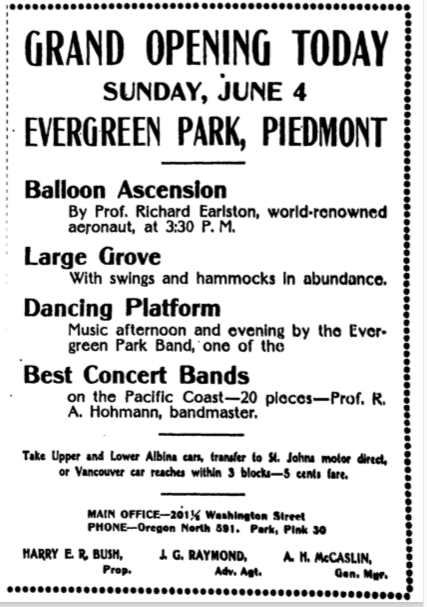
\includegraphics{images/image23.png}
\caption{alt\_text}
\end{figure}

\begin{verbatim}
March 30 1961
\end{verbatim}

{\textgreater\textgreater\textgreater\textgreater\textgreater{} gd2md-html alert: inline image link here (to images/image24.png). Store image on your image server and adjust path/filename/extension if necessary. }(Back to top)(Next alert){\textgreater\textgreater\textgreater\textgreater\textgreater{} }

\begin{figure}
\centering
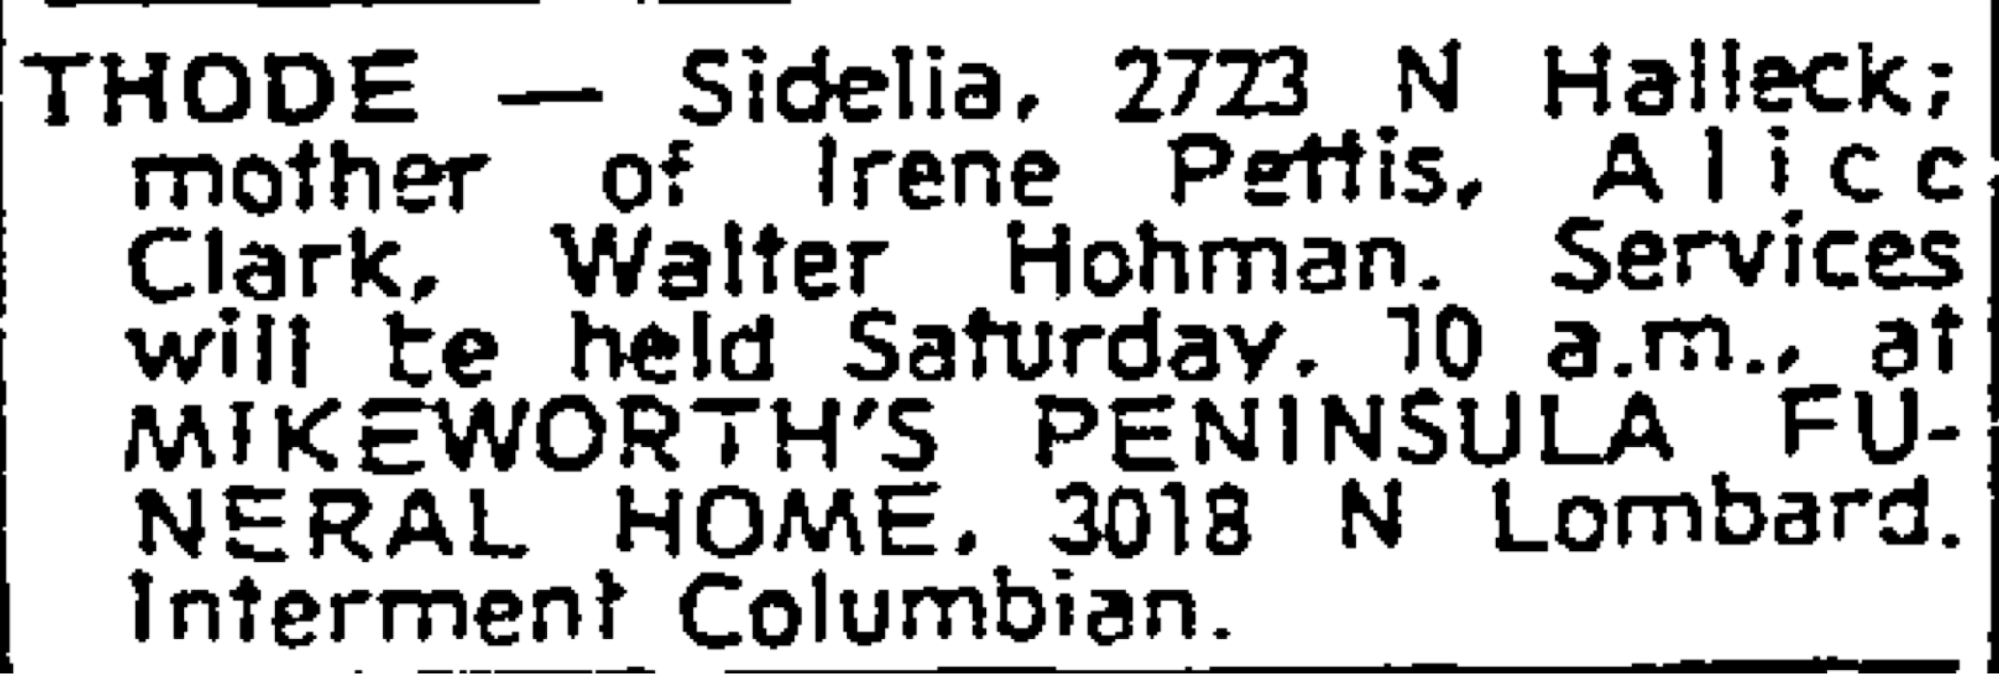
\includegraphics{images/image24.png}
\caption{alt\_text}
\end{figure}

\begin{verbatim}
September 6, 1964
\end{verbatim}

When we bought the house in 2014 the knotty pine kitchen and cedar bathroom were still there, and were probably pretty much unchanged over 50 years. We did not know how fast to get rid of them.

We see the price of the house increasing from about \$ 10K to about \$15K over a three-year period. The sale did not go well, I guess, and it looks like they hired a real estate agent in the early seventies. You'll see that in the next section, because the real estate agent actually bought the house in 1971. Max and Marguerite Boehm moved to Lake Oswego.

Jean C. Baldwin and Doc F. Baldwin

On March 11, 1971 Max D. Boehm and Marguerite E. Boehm sold the property to Doc F. Baldwin and Jean C. Baldwin for \$ 16,750. The Baldwins worked for, or owned, Bucher Real Estate. Again, it is unclear if they ever lived in the house. They may have rented it out. The ads became more glossy. And we do see the price going up, from \$ 18K in 1971 to \$ 33K in 1976.

\begin{verbatim}
[https://drive.google.com/file/d/1MCQHUf5CBzSPZjhBAi8rwwdtx9BDGr7B](https://drive.google.com/file/d/1MCQHUf5CBzSPZjhBAi8rwwdtx9BDGr7B)
\end{verbatim}

{\textgreater\textgreater\textgreater\textgreater\textgreater{} gd2md-html alert: inline image link here (to images/image25.png). Store image on your image server and adjust path/filename/extension if necessary. }(Back to top)(Next alert){\textgreater\textgreater\textgreater\textgreater\textgreater{} }

\begin{figure}
\centering
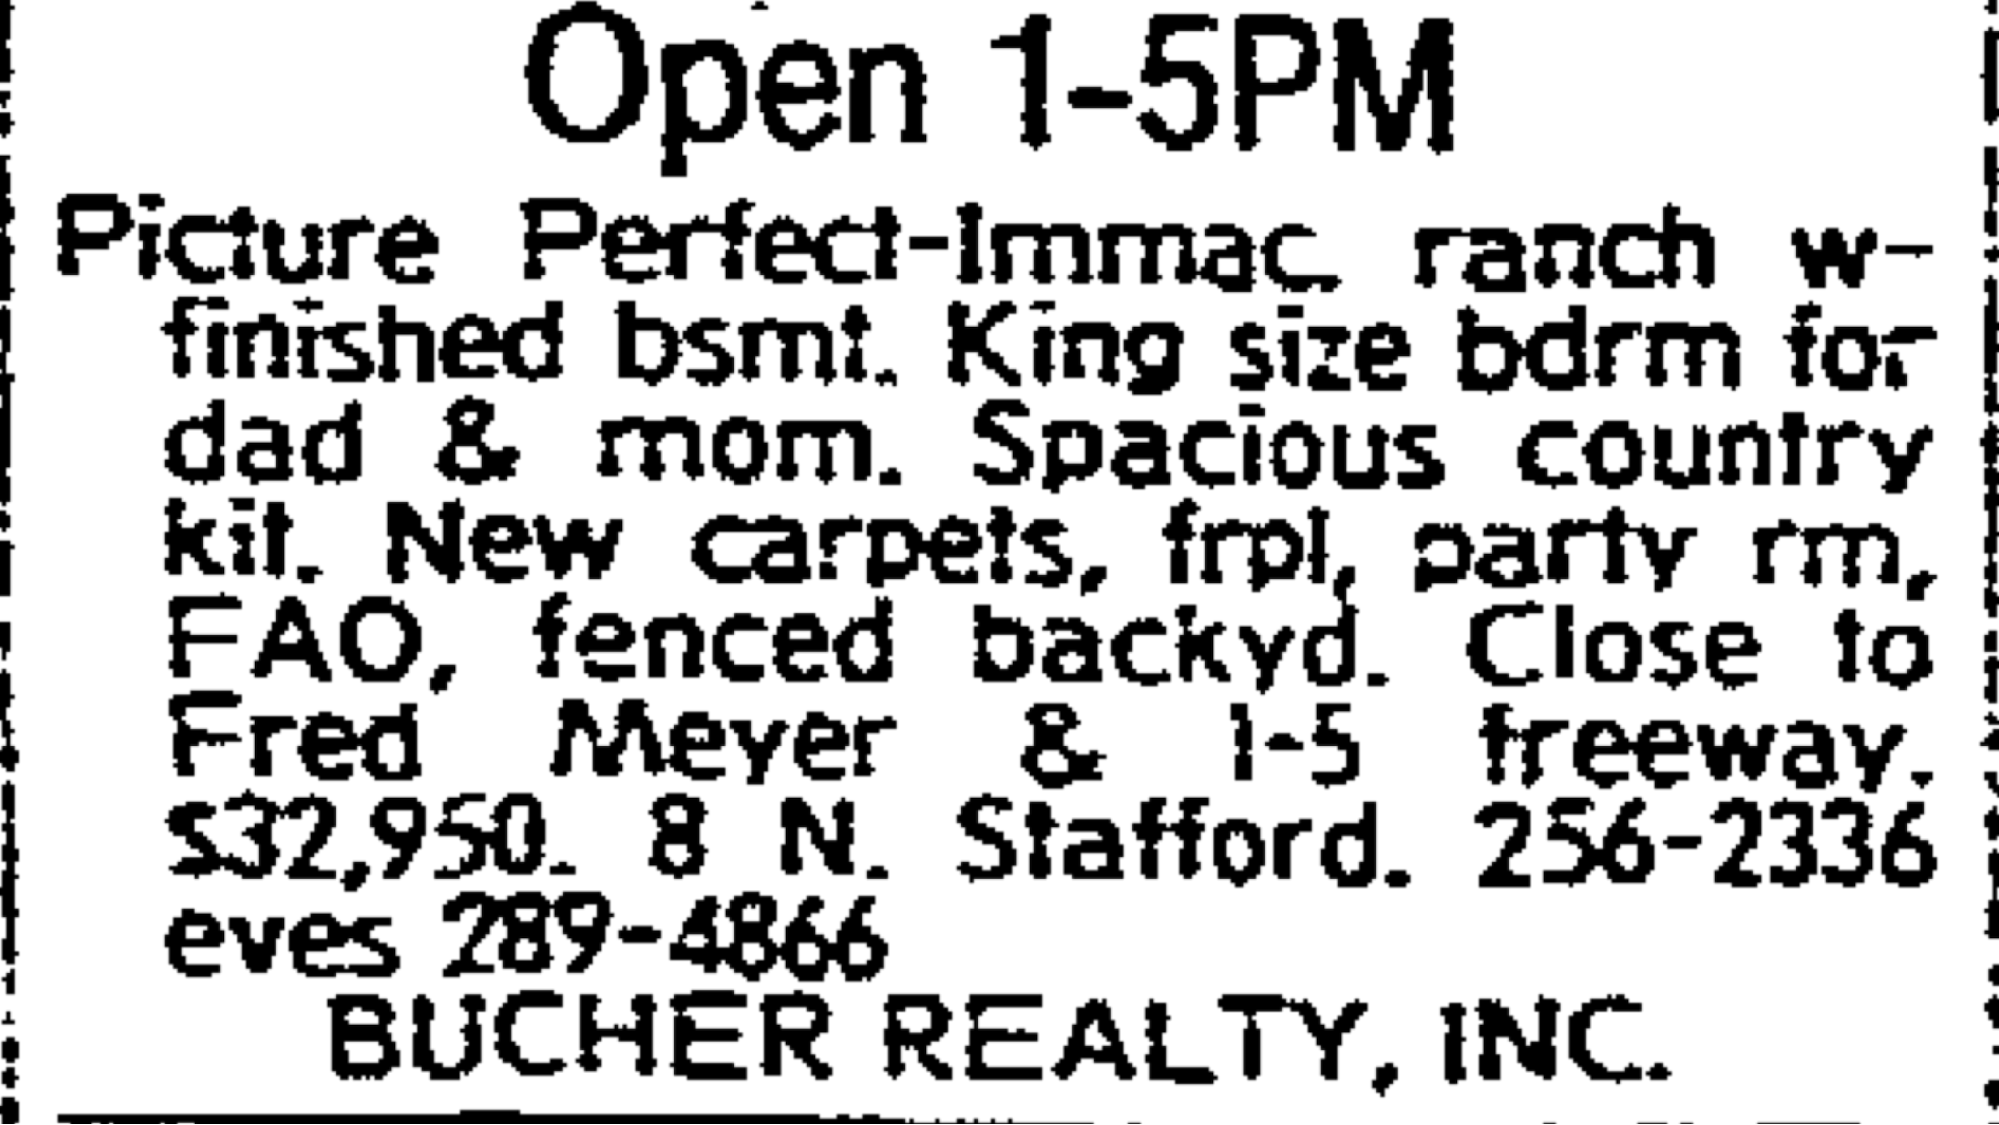
\includegraphics{images/image25.png}
\caption{alt\_text}
\end{figure}

March 7, 1971

{\textgreater\textgreater\textgreater\textgreater\textgreater{} gd2md-html alert: inline image link here (to images/image26.png). Store image on your image server and adjust path/filename/extension if necessary. }(Back to top)(Next alert){\textgreater\textgreater\textgreater\textgreater\textgreater{} }

\begin{figure}
\centering
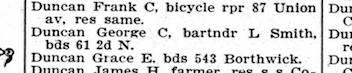
\includegraphics{images/image26.png}
\caption{alt\_text}
\end{figure}

March 14, 1971

{\textgreater\textgreater\textgreater\textgreater\textgreater{} gd2md-html alert: inline image link here (to images/image27.png). Store image on your image server and adjust path/filename/extension if necessary. }(Back to top)(Next alert){\textgreater\textgreater\textgreater\textgreater\textgreater{} }

\begin{figure}
\centering
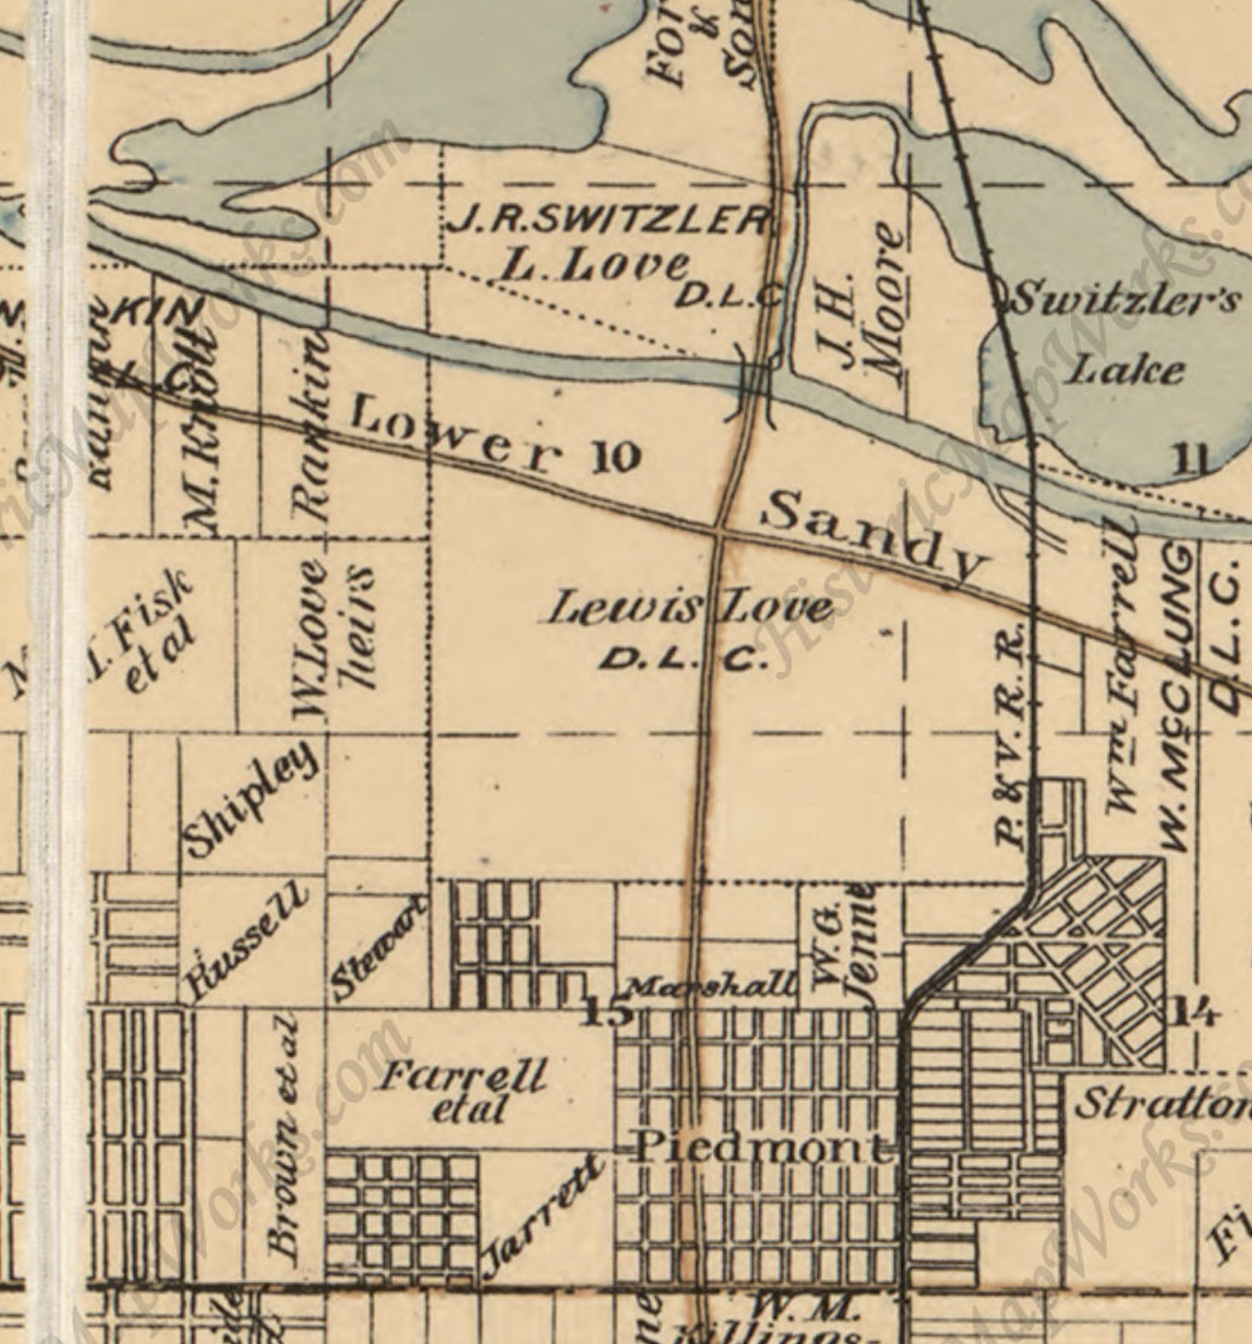
\includegraphics{images/image27.png}
\caption{alt\_text}
\end{figure}

October 3, 1976

The wood panelling in the bathroom and the kitchen, which we removed as quickly as possible, in 2014, is announced proudly as a redeeming feature of the house. So is the closeness to Holy Redeemer. The 30 ft living room is still there. I assume the party room was the basement or part of the basement. The section on modifications below shows us that the Boehms put in the new (oil) furnace in 1949 and the new fireplace in 1952.

Lan Thi Nguyen and Dong Van Nguyen

The Baldwins sold the house on December 10, 1976 to Lan Thi Nguyen and Dong Van Nguyen, husband and wife, for \$ 29,000.

\url{https://drive.google.com/open?id=1jj6mVZRq6Poxo22lVSQCSEvJ_NkdWyCN}

The Nguyens lived there for more than 30 years, definitely setting the record. To find out more about their stay is complicated, for various reasons. Most importantly, the Nguyens were, or are, of Vietnamese descent, and Wikipedia tells us that up to 40\% of the people in Vietnam have Nguyen as their last name. Because there is a substantial Vietnamese community in Portland, there are consequently many people named Nguyen. The junk mail we are still getting indicates there were more than two Nguyens living in the house over the 1976-2014 period, but the composition of the family and their relationships remain unclear.

What we can figure out, using the Multnomah County registrar's database, are the various transactions and deeds the Nguyens entered into in order to finance buying and maintaining the house. There are multiple deeds of trust, indicating various home equity loans and mortgages. Eventually, it seems, the Nguyens got caught up in the subprime mortgage crisis of 2007 and were forced out of the house by foreclosure.

For yours and mine information, here is the definition of a deed of trust from The \href{https://www.law.cornell.edu/wex/deed_of_trust}{Legal Information Institute at the Cornell Law School}.

\begin{verbatim}
_A Deed of Trust is a type of [secured](https://www.law.cornell.edu/wex/secured_transactions) [real-estate](https://www.law.cornell.edu/wex/real_property) [transaction](https://www.law.cornell.edu/wex/secured_transactions) that some states use instead of [mortgages](https://www.law.cornell.edu/wex/mortgage). A deed of trust involves three parties: a lender, a borrower, and a trustee. The lender gives the borrower money. In exchange, the borrower gives the lender one or more [promissory notes](https://www.law.cornell.edu/wex/negotiable_instruments). As security for the [promissory notes](https://www.law.cornell.edu/wex/negotiable_instruments), the borrower transfers a [real property](https://www.law.cornell.edu/wex/real_property) interest to a third-party trustee. Should the borrower [default](https://www.law.cornell.edu/wex/default) on the terms of her loan, the trustee may take full control of the property to correct the borrower's [default](https://www.law.cornell.edu/wex/default)._


_Usually, the trustee is a title company. In most states, the borrower actually transfers legal title to the trustee, who holds the property in trust for the use and benefit of the borrower. In other states, the trustee merely holds a [lien](https://www.law.cornell.edu/wex/lien) on the property. Deeds of trust almost always include a [power-of-sale clause](https://www.law.cornell.edu/wex/power-of-sale_clause), which allows the trustee to conduct a [non-judicial foreclosure](https://www.law.cornell.edu/wex/non-judicial_foreclosure) - that is, sell the property without first getting a court order. _
\end{verbatim}

The first one is dated December 10, 1976, the second June 25, 1979, and the third October 21, 1982, and the fourth on July 10, 2006. In the first two the lender is the Far West Savings and Loan Association, for the third it is the Small Business Administration, and for the fourth one it is the Taylor, Bean and Whitaker Mortgage Corporation. The first three have Lan Thi Nguyen and Dong Van Nguyen as the borrowers, for the fourth one it is Lan Thi Nguyen, an unmarried woman.

The 2006 loan, for \$ 224,000, looks like a predatory loan, and was made, of course, just before the start of the subprime crisis. The lender is somewhat suspect, to say the least. From \href{https://en.wikipedia.org/wiki/Taylor,_Bean_\%26_Whitaker}{Wikipedia}

\begin{verbatim}
**_Taylor, Bean & Whitaker was a top-10 wholesale [mortgage lending](https://en.wikipedia.org/wiki/Mortgage_loan) firm in the [United States](https://en.wikipedia.org/wiki/United_States), the fifth-largest issuer of [Government National Mortgage Association](https://en.wikipedia.org/wiki/Government_National_Mortgage_Association) (GNMA or Ginnie Mae) securities. Their slogan was "Perfecting the Art of Mortgage Lending"._**


_On August 5, 2009, following a raid by the Special Inspector General of the Troubled Asset Relief Program (SIGTARP) and suspension by the [Federal Housing Administration](https://en.wikipedia.org/wiki/Federal_Housing_Administration) from issuing FHA mortgage loans and Ginnie Mae mortgage-backed securities, it ceased business operations. In April 2011, its majority owner was convicted of 14 counts of securities, bank, and wire fraud and conspiracy to commit fraud, and sentenced to 30 years in federal prison._
\end{verbatim}

It is clear that Lan Thi Nguyen could not make the mortgage payments, and consequently lost the house. I may still work out the details, but the end result is clear.

On August 18, 2014 Nicole and Jan de Leeuw bought the property from the Federal Home Loan Mortgage Corporation for \$ 250,000. In 2021 the house will be 100 years old.

Modifications

To track modifications to the original home built by the Radditz family in 1921 we have to go to the archive of the City's Bureau of Development Services. We have only found permits applied for and issued to Max Boehm. Here is the 1949 permit application for the new oil furnace, with a 275 gallon fuel tank (which may still be in the ground somewhere, although the furnace is long gone).

{\textgreater\textgreater\textgreater\textgreater\textgreater{} gd2md-html alert: inline image link here (to images/image28.jpg). Store image on your image server and adjust path/filename/extension if necessary. }(Back to top)(Next alert){\textgreater\textgreater\textgreater\textgreater\textgreater{} }

\begin{figure}
\centering
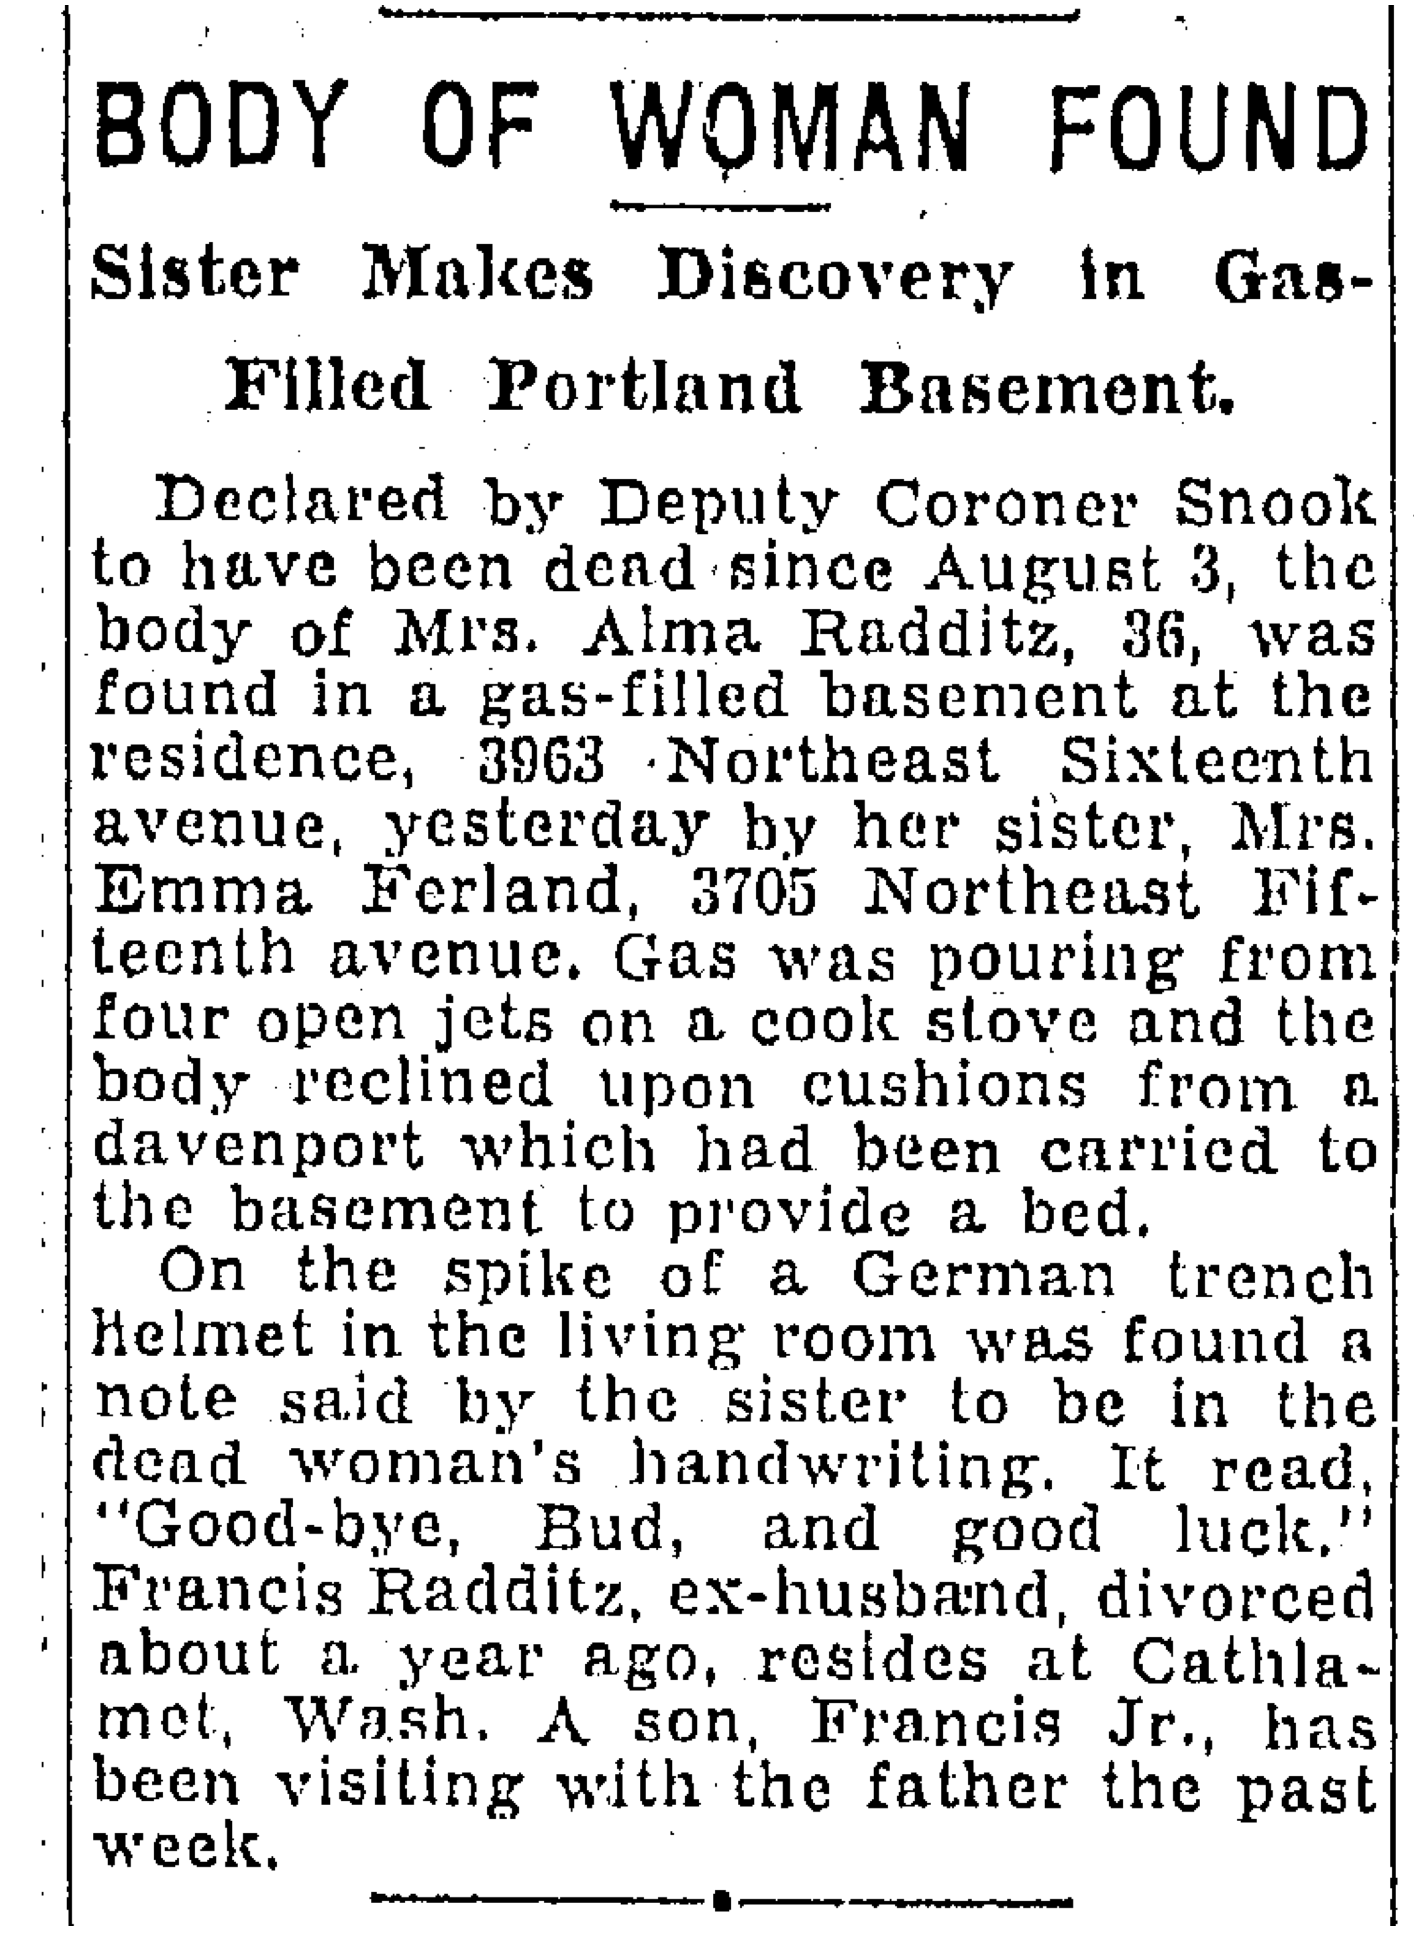
\includegraphics{images/image28.jpg}
\caption{alt\_text}
\end{figure}

There are some additional permits with more consequential. On July 3, 1950 Boehm filed for a permit to build an extension of 7333 N. Williams on the west side. This included an enclosed back porch and a stairway to the basement. Costs are estimated to be \$ 500.

\url{https://drive.google.com/open?id=1Ew6UqQXh9zC9aZyat4SYsXXON-0_swUF}

Next is an application of March 14, 1952 for a ``\emph{new outside fireplace extended to solid ground}''. The accompanying plan seems to include a new front porch on Stafford, although the address is still 7333 N. Williams. Costs of the alterations are estimated as \$ 2,500, and Boehm will do the work himself.

\url{https://drive.google.com/open?id=1b08jj8gqZJygOTzQwAtVlUAljCwtbT6R}

The report of a BDS building inspector of August 17, 1956 documents that Boehm built 30 feet of 6'3'\,' high cedar fence, costs \$ 30, and that the building was finished before the permit was issued. The address given in 1956 was 8 N. Stafford.

\url{https://drive.google.com/open?id=1H8nQMnuRZyKw2AccGyUkg8POoF_lmfRX}

An application by Bromley Masonry, from November 21, 1962, asks for a permit for ``\emph{repair of chimney damaged by Columbus Day storm}'' at 8 N. Stafford, with the Boehm family still in residence. The costs are \$ 132.04.

\url{https://drive.google.com/open?id=1ziFcImzPOfz6U_EEAbNg6eaQqPqHvLFz}

I am still trying to nail down when exactly the street address changed from 7333 N. Williams to 8 N. Stafford. For now it seems that it was certainly between 1952 and 1956, and closer to 1952.

It seems the Nguyen family did not make any substantial changes. When we came in 2014 the house had been empty for a couple of years and was somewhat neglected. In the five years since 2014 we completely changed the kitchen, the bathroom, the bedrooms, the basement, the fencing, the yard, the siding, the garage, the porch, the furnace, the chimney, the fireplace, the back doors. But the overall structure is still classical 1920's Radditz, with 1950's Boehm extensions.

\end{document}
